\documentclass[11pt,a4paper]{article}

\usepackage[T1]{fontenc}
\usepackage[utf8]{inputenc}
\usepackage{lmodern}
\usepackage{microtype}
\usepackage[margin=2.5cm]{geometry}
\usepackage{graphicx}
\usepackage{xcolor}
\usepackage{booktabs}
\usepackage{amsmath}
\usepackage{enumitem}
\usepackage{url}
\usepackage{tikz}
\usetikzlibrary{positioning}
\usepackage[hidelinks]{hyperref}

\newcommand{\figdir}{../../reports/figures/}
\graphicspath{{../../reports/figures/}}

% Visible box for content a team member still has to supply.
\newcommand{\todobox}[1]{%
  \par\medskip\noindent
  \fcolorbox{red!70!black}{red!4}{%
    \parbox{\dimexpr\linewidth-2\fboxsep-2\fboxrule\relax}{%
      \textbf{\textcolor{red!70!black}{TODO}}\par\smallskip #1}}%
  \par\medskip}

% Include a figure from reports/figures/ if it exists, otherwise show a TODO box.
% Optional first argument: the width (default 0.85\linewidth).
\newcommand{\safefigure}[4][0.85\linewidth]{%
  \IfFileExists{\figdir #2}{%
    \begin{figure}[htbp]
      \centering
      \includegraphics[width=#1]{#2}
      \caption{#3}
      \label{#4}
    \end{figure}%
  }{%
    \todobox{Missing figure \texttt{reports/figures/\detokenize{#2}}: #3}%
  }}

\begin{document}

% Long \texttt paths cannot be hyphenated; let the spaces stretch instead of
% running into the margin.
\setlength{\emergencystretch}{6em}

\pagenumbering{alph}
\begin{titlepage}
  \centering
  \vspace*{3cm}
  {\Huge\bfseries SignBridge PK\par}
  \vspace{0.8cm}
  {\Large Static Letter Recognition in American Sign Language\par}
  \vspace{0.3cm}
  {\large A first step towards Pakistan Sign Language\par}
  \vspace{1.5cm}
  {\large Project Report\par}
  \vspace{0.3cm}
  {\large November 2026\par}
  \vspace{2.2cm}
  {\large\bfseries Team\par}
  \vspace{0.4cm}
  \begin{tabular}{ll}
    Aliza  & Data Lead \\
    Fatima & Model Lead \\
    Anas   & App and Integration Lead \\
  \end{tabular}
  \vfill
\end{titlepage}

\pagenumbering{roman}
\begin{abstract}
\noindent
People who use Pakistan Sign Language (PSL) and people who do not know it often have no shared language. SignBridge PK is a first step towards a tool that reads a single photograph of a hand and returns the most likely letter. We have no PSL photographs yet, so every model in this report is trained and tested on the American Sign Language (ASL) alphabet; the results describe ASL, not PSL. We built two kinds of recogniser for the 26 letters A to Z: a convolutional network (MobileNetV2) that reads the image, and support vector machine, random forest and neural network classifiers that read 21 hand landmarks found by MediaPipe. The data was split by groups of look-alike images, so that near-identical frames do not appear in both training and test. On the 1{,}560 test images the CNN reaches 0.9795 accuracy and 0.9795 macro-F1. The landmark models can answer only the 1{,}090 test images (69.9\%) in which a hand was detected; on those images the CNN scores 0.9780 and the chosen SVM 0.9688. These scores are optimistic. Many test images have a near-identical training image of the same letter (70.0\% within 8 bits of an image hash), the data has no signer labels, and we made no claim about fairness across people. The scores are not an estimate of accuracy on new signers or on PSL. The next step is to collect PSL photographs with signer labels and test on people not seen in training.
\end{abstract}

\tableofcontents
\clearpage
\pagenumbering{arabic}

\section{Introduction}
\label{sec:introduction}

People who communicate in Pakistan Sign Language (PSL) and people who do not know it often cannot talk to each other without an interpreter, pen and paper, or improvised gestures (Section~\ref{sec:problem}). SignBridge PK is a student project that takes a first, deliberately small step towards a tool that helps: given one photograph of one hand, it returns the most likely letter and how confident it is. Letters are the natural first target because fingerspelling is used for names, addresses and technical terms, which are exactly the words that improvised gestures cannot carry~\cite{pslcfrt}.

\subsection{What This Report Covers}

The report defines the problem, the intended users and the data, and it cleans and explores the image data (Sections~\ref{sec:problem} to~\ref{sec:eda}). It then builds two recognisers, splits the data so that the test set is a fair test, and evaluates them (Sections~\ref{sec:cnn} to~\ref{sec:limitations}). Finally, the trained models are used in a local web application that takes an uploaded or webcam image and shows the three most likely letters from the CNN or the landmark SVM, with a landmark overlay, a clear message when no hand is found, and a visible note that the models were trained on ASL letters. The report ends with sample predictions, a section that records why the planned user test of the application was not carried out, and conclusions.

\subsection{An Important Limit: ASL, Not PSL}

We have collected no PSL photographs. The only large labelled alphabet dataset available to us is the American Sign Language (ASL) alphabet dataset~\cite{asl_alphabet_kaggle}, and ASL and PSL are different sign languages with different hand shapes. We therefore used ASL as a practice set to build and compare the whole pipeline. Every score in this report describes ASL. None of it shows how well a model would recognise PSL.

\subsection{What We Built}

\begin{itemize}
  \item \textbf{Two recognisers.} A convolutional network based on MobileNetV2~\cite{sandler2018mobilenetv2} reads the pixels of the image (Section~\ref{sec:cnn}). A second family first finds 21 hand landmarks with MediaPipe~\cite{zhang2020mediapipe} and then classifies them with a support vector machine~\cite{cortes1995svm}, a random forest or a small neural network (Section~\ref{sec:landmark-models}). The landmark models answer only when a hand is detected.
  \item \textbf{A fair split.} The ASL images are video frames, so a random split would place almost identical frames in training and test. We split by groups of look-alike images (Section~\ref{sec:validation}).
  \item \textbf{Honest evaluation.} We report accuracy, macro-F1, AUC-ROC and the confusion matrix, compare the two families on the same images, analyse the mistakes and check how the CNN behaves by image brightness, blur and hand detection (Sections~\ref{sec:metrics} to~\ref{sec:bias-check}).
\end{itemize}

\subsection{What the Results Do and Do Not Show}

The CNN scores close to 100\% on our test set. We do not read this as success. Many test images have a near-identical training image of the same letter, and the dataset has no signer labels, so the scores are optimistic and are not an estimate of accuracy on new people (Sections~\ref{sec:read-scores} and~\ref{sec:limitations}). The report states these limits wherever a score is given.

\section{Related Work}
\label{sec:related-work}

This section is short on purpose. It covers only the sources we have read and cited in this report, and it does not claim a survey of the field. We did not reproduce any of these works, and we do not compare their scores with ours, because they use different data and evaluation protocols.

\subsection{PSL Data}

Public PSL data is limited~\cite{colorglove_psl}, and the datasets we found differ in what they contain. One captured 40 images for each hand configuration of the Urdu alphabet~\cite{imran2021psl}. UAlpha40 contains 36 static signs as JPG images and 4 dynamic signs as MP4 videos, under a CC BY 4.0 licence~\cite{sajid2025ualpha40}. A Kaggle dataset holds 37 Urdu alphabet signs performed by 9 non-expert subjects~\cite{butt_psl_kaggle}. PSL-CFRT is a benchmark multi-view dataset for continuous fingerspelling recognition and translation~\cite{pslcfrt}. The sources disagree on the number of letters, from 34 to 37, and we have not verified a letter list of our own (Section~\ref{sec:problem}).

\subsection{PSL Recognition}

Published PSL work includes automatic recognition of the hand configurations of the Urdu alphabet through machine learning~\cite{imran2021psl} and recognition of PSL alphabets from geometrical features with the help of a coloured glove~\cite{colorglove_psl}. Our landmark models are related in spirit to the geometrical-feature approach, since they classify the positions of hand points instead of the pixels; they need no glove, because MediaPipe finds the landmarks in an ordinary photograph. We note this only as a similarity of idea. We did not compare the two methods.

\subsection{ASL Baseline}

Because no large PSL set was available to us, we trained on the ASL Alphabet dataset on Kaggle~\cite{asl_alphabet_kaggle}, published under the GPL~2 licence. It is the most accessible large alphabet dataset we found, and it is made of frames from short recordings with no signer labels. This is why the split in Section~\ref{sec:validation} groups look-alike images, and why our scores are optimistic.

\subsection{What We Add}

Our contribution is not a new method. It is a careful, honest evaluation of two standard recognisers: a split that is aware of near-duplicate frames, a comparison on the same images, an analysis of the mistakes, and a plain statement of what the scores do not show. We make no claim about PSL.


\part{Problem Definition and Data Acquisition}

\section{Problem Statement}
\label{sec:problem}

\subsection{The Communication Barrier}

People who communicate in Pakistan Sign Language (PSL) and people who do not know it often have no shared language. Published work on PSL describes this as a communication gap between the deaf and non-deaf communities~\cite{imran2021psl}. In everyday settings such as a classroom, a shop, a clinic or a family gathering, a conversation between a signer and a non-signer then depends on a human interpreter, on writing things down, or on improvised gestures. Interpreters are not always available. Writing is slow and depends on both people sharing a written language. Gestures break down as soon as the message becomes specific, for example a person's name or an address.

Non-signers who want to meet signers halfway, such as relatives, classmates and teachers, need a way to learn and practise signs, and to check whether they are reading or producing a sign correctly.

\subsection{Limited PSL Data}

Publicly available PSL datasets are limited~\cite{colorglove_psl}. The ones we found differ in what they contain: one captured 40 images for each hand configuration of the Urdu alphabet~\cite{imran2021psl}; UAlpha40 contains 36 static signs as JPG images and 4 dynamic signs as MP4 videos~\cite{sajid2025ualpha40}; and a Kaggle dataset contains 37 Urdu alphabet signs performed by 9 non-expert subjects~\cite{butt_psl_kaggle}. The large, labelled alphabet dataset we could download for a baseline is an American Sign Language (ASL) dataset~\cite{asl_alphabet_kaggle}, not a PSL one. A model trained only on ASL cannot be used for PSL, because the two are different sign languages with different signs.

\subsection{Why Start with Letters}

In PSL, fingerspelling represents the letters of the Urdu alphabet~\cite{colorglove_psl}, and it is used for proper names, technical terms, addresses and uncommon words~\cite{pslcfrt}. A tool that recognises individual letters therefore helps exactly in the situations where improvised gestures fail.

Letters are also a sensible first step for a technical reason. Each static letter is a single hand shape that can be captured in one image, the set of classes is small and fixed, and every prediction can be checked against a known answer. Recognising words, sentences or signs that involve movement needs sequences of frames and a much larger dataset, which is outside what one course project can build and evaluate properly.

\subsection{Which Letters}

There is no single agreed list of PSL letters to recognise. The published sources above report different numbers of signs: 36 static signs~\cite{sajid2025ualpha40}, 34 static alphabets~\cite{colorglove_psl} and 37 alphabet signs~\cite{butt_psl_kaggle}; together they place the PSL letter set at 34 to 37 letters. We have not yet verified a letter list ourselves. The PSL letter set will therefore be fixed later from a cited source and checked with a PSL user. The current label map, with the 26 letters A to Z, fits the ASL baseline only.

\subsection{Scope}

This project covers \textbf{static letter signs only}. The system receives a single image of one hand and returns the most likely letters with their confidence. It does not recognise motion-based signs, words or sentences, and it does not translate speech or text into signs.

\section{Target Audience}
\label{sec:audience}

SignBridge PK is a \textbf{learning and practice aid}. It is not a replacement for a qualified PSL interpreter and must not be used where an accurate interpretation matters, such as medical, legal or official settings. The groups below are the intended users and what each of them needs from the tool. No user testing has been carried out yet; these needs describe the design goals, not observed results.

\begin{description}[style=nextline, leftmargin=1.5em]
  \item[Learners of PSL]
    People starting to learn PSL need to practise letter signs on their own and get immediate feedback on whether their hand shape is recognised. They need clear output (the predicted letter and how confident the system is) and a way to retry quickly.

  \item[Family members and classmates of PSL users]
    Hearing people who live, study or work with a PSL user may want to learn fingerspelling so they can spell names and unfamiliar words. They need a tool that runs on an ordinary laptop with a webcam, without special hardware or setup.

  \item[Teachers]
    Teachers working with deaf or hard-of-hearing students, or teaching PSL, need a simple way to demonstrate letter signs and let students practise between lessons. They need the tool to behave consistently and to show when it is unsure instead of giving a confident wrong answer.

  \item[The PSL community]
    Signers who want to practise or check letter signs, or help others learn, need the tool to respect PSL as its own language rather than treating it as a variant of ASL. They also need their images handled with care: our own data is to be collected only from consenting volunteers and is not published in the code repository.
\end{description}

\subsection{What the Tool Does Not Do}

\begin{itemize}
  \item It does not interpret conversations, words or sentences.
  \item It does not recognise signs that involve movement.
  \item It does not claim to work equally well for every signer, hand, lighting condition or camera. How performance varies across these factors is measured in later work.
\end{itemize}

\section{AI Justification}
\label{sec:ai-justification}

The task is to decide which letter of the alphabet a hand shows in a webcam image. This section explains why we use machine learning for this decision instead of hand-written rules. It contains no accuracy numbers; the results are reported later in this report.

\subsection{The Variation a Rule Would Have to Handle}

\textbf{Differences between people.} Hands differ in size, finger length and skin tone, and each person forms the same letter a little differently: how far a finger is bent, how wide the fingers are spread, where the thumb rests. Two correct examples of the same letter are therefore never identical.

\textbf{Differences in how the image is captured.} Lighting, background, camera angle and distance change the image even when the sign is the same. In the five ASL baseline sample images where hand detection failed (Section~\ref{sec:feature-results}), the picture is low resolution, the hand fills most of the frame, and in most of them it touches or crosses the edge of the picture.

\textbf{Letters that look alike.} Some letters differ only slightly. In the ASL baseline, A, E, M, N and S are all closed-hand shapes that differ mainly in where the thumb sits relative to the other fingers, and all five are in our sample. A small change in one finger decides the class, while a change of the same size caused by a different person or a different camera angle must be ignored.

\subsection{Why Hand-Written Rules Are Impractical}

A rule-based recogniser would first have to locate the hand and its fingers, then measure quantities such as the bend angle of each finger and the position of the thumb, and then compare them with fixed thresholds written for each letter, for example ``the index finger counts as straight if its bend angle is below a limit''. This breaks down under the variation above in three ways:
\begin{itemize}[leftmargin=1.5em, topsep=2pt]
  \item A threshold that fits one person's hand can fail on another's. One limit cannot suit large and small hands, or different ways of forming the letter.
  \item For letters that look alike, the thresholds that separate them lie close together, so small measurement errors caused by the camera angle or image noise can flip the result.
  \item Every new source of variation, such as a new camera, new lighting or new volunteers, means re-tuning thresholds by hand, and tuning the thresholds of one letter can break another.
\end{itemize}
Even the first step, finding the hand in the image, is hard to write as rules. Our pipeline uses a ready-made learned model, the MediaPipe hand landmarker, for that step (Section~\ref{sec:feature-strategy}). We have not built a rule-based recogniser on the landmarks, so we make no claim about how well one would perform. The argument here is about the effort and fragility of maintaining many hand-tuned thresholds, not about a measured result.

\subsection{What a Learned Model Provides}

A learned model replaces the hand-written thresholds with decision boundaries found from labelled examples. If the training examples come from many people and conditions, the model sees the variation instead of having it described in rules, and new examples can be added by retraining instead of re-tuning by hand. Normalising the landmarks (Section~\ref{sec:feature-strategy}) removes only the position and size of the hand; the remaining variation is what the classifier has to learn.

A learned model can also be evaluated honestly. The manifest builder records the volunteer and the split of every PSL image, so once PSL photos are collected the model can be tested on people it has not seen during training, which is the situation a real user creates.

The approach has a limit: a learned model handles only the variation present in its training data. If the volunteers are few or not varied, the model may fail on other people. This is why the PSL data collection and the bias analysis by the data team matter for the result.
\section{Data Collection}
\label{sec:data-collection}

\subsection{ASL Baseline Data}

The baseline dataset is the ``ASL Alphabet'' dataset on Kaggle~\cite{asl_alphabet_kaggle}, published under the GPL~2 license. It is downloaded with \texttt{data\_scripts/download\_data.py}, which reads the dataset identifier and the destination folder from \texttt{configs/data.yaml}. The images are never committed to the repository.

After download, the training folder contains 29 classes with 3{,}000 JPEG images each, 87{,}000 images in total: the letters A to Z and three extra classes stored as \texttt{del}, \texttt{nothing} and \texttt{space}. The separate test folder contains 28 images. These counts come from listing the downloaded files.

The dataset is American Sign Language. It is used only to build and test the data pipeline and as a comparison point; it is not PSL data.

\subsection{PSL Data Collected by the Team}

The PSL photos are collected by the team under a written protocol, \path{docs/data_collection_protocol.md}.

\begin{itemize}
  \item \textbf{Scope:} static letter signs only, with no motion, words or sentences.
  \item \textbf{Volunteers:} the aim is 5 to 10 volunteers. Each gets an anonymous ID (\texttt{p01}, \texttt{p02}, \ldots); no names or contact details are stored with the photos or in the repository.
  \item \textbf{Consent:} before shooting, a short consent note is read to each volunteer. It says the photos are used only for this university project, asks the volunteer to keep their face out of the frame, and explains that the photos are stored under an anonymous ID, are not uploaded to GitHub and are not shared beyond the project team and course assessors, and that the volunteer can stop at any time and ask for the photos to be deleted. Consent is recorded per volunteer ID in a private sheet kept outside the repository; the same sheet is the only link between an ID and a person, and it exists only so a volunteer can ask for their photos to be deleted.
  \item \textbf{What is captured:} every letter for every volunteer, with the right hand by default, under three lighting conditions (normal, dim, bright) and two backgrounds (plain, cluttered), with a proposed minimum of 10 images per letter per volunteer, spread across these variations.
  \item \textbf{Skin tone group (optional):} the consent note explains that we would like to check whether the recognizer works equally well for different people, and asks the volunteer to choose a broad skin tone group, or to skip the question. The answer is self-reported and never guessed from a photo. It is kept only in the private sheet, not in the committed \texttt{manifest.csv}, and is joined to results by volunteer ID on a local machine for the bias analysis. Only aggregate results are committed, a group with fewer than three volunteers is never reported, and, because the sample is small, the bias check is descriptive.
  \item \textbf{Storage:} photos are saved outside Git in \texttt{data/raw/psl} with file names of the form \texttt{p03\_alif\_dim\_plain\_004.jpg}: volunteer, letter label, lighting, background and image number. The scripts read these facts from the file name.
\end{itemize}

The script \texttt{data\_scripts/build\_manifest.py} builds \texttt{data/processed/manifest.csv} from these photos, reading volunteer, letter, lighting and background from each file name. It assigns whole volunteers, never single images, to training, validation and test, and its tests fail if any volunteer appears in more than one split.

\subsection{Status of the PSL Collection}

At the time of writing, no PSL photos have been collected: the folder \texttt{data/raw/psl} does not exist yet, so the dataset contains 0 volunteers and 0 images. The letter set has not been confirmed, and no PSL dictionary, deaf association or PSL user has yet been consulted to check the sign shapes. These two points must be settled before collection starts, and the protocol marks the corresponding fields as still to be decided rather than guessing them.

What exists is the pipeline. The collection protocol is written, and the manifest builder and the cleaning and EDA scripts have been built and tested. The cleaning and EDA scripts have been run on a sample of the ASL baseline (2{,}900 images, 100 per class, 29 classes). PSL collection has not started, and the dataset hosting link will be added once PSL data exists.

\section{Data Cleaning}
\label{sec:data-cleaning}

The cleaning script \texttt{data\_scripts/clean/clean\_images.py} checks every image of one dataset (the ASL baseline or the PSL photos) and writes its findings to a report. It never deletes or changes an image file: it only flags problems and counts them. All thresholds are read from \texttt{configs/data.yaml}, section \texttt{quality}, so none is hard-coded. For the ASL baseline only the labelled training folder is cleaned; the separate test folder is left out.

\subsection{Cleaning Steps}

The steps run in this order, and each step looks only at the images that earlier steps kept.
\begin{enumerate}
  \item \textbf{Missing data: unreadable files and missing labels.} An image is flagged if the file is empty, corrupt or cannot be decoded as an image. An image also counts as missing its label if an ASL image lies outside a class folder, or if a PSL file name does not follow the collection protocol, so that no label can be read from it.
  \item \textbf{Exact duplicates.} The SHA-256 hash of each file's bytes is computed. Files with identical hashes are exact copies; the first copy in path order is kept and later copies are flagged. This check runs across all classes, so an identical file stored under two labels is also found.
  \item \textbf{Near-duplicates.} Each image is converted to grayscale and shrunk to $9 \times 8$ pixels, and each pixel is compared with its right neighbour, which gives a 64-bit difference hash. Two images of the same class whose hashes differ in at most \texttt{quality.near\_duplicate\_distance} bits are near-duplicates; the first is kept and the later one is flagged. Each flagged image records the path of the image it duplicates, so the pairs can be checked by eye.
  \item \textbf{Outliers.} An image is flagged if its shorter side is below \texttt{quality.min\_side} pixels; if it is blurry, meaning the variance of its Laplacian is below \texttt{quality.blur\_threshold}; or if its mean grayscale value is below \texttt{quality.brightness\_min} (too dark) or above \texttt{quality.brightness\_max} (too bright).
\end{enumerate}

\subsection{Outputs}

The script writes three files. The per-image report (path, dataset, class, volunteer, size, hash, blur score, brightness and every flag) is saved in \texttt{data/interim/} and is not committed. The counts per class after each step are saved in \texttt{reports/cleaning\_summary.csv}, and a table of the totals per dataset is saved as \texttt{reports/cleaning\_summary\_table.tex} and included below. Running the script again for one dataset replaces only that dataset's rows. For a quick run, the option \texttt{-{}-limit-per-class} cleans a random sample of each class, chosen with the \texttt{seed} from the configuration so the same images are chosen every time.

\subsection{Class Names}

The cleaning outputs keep the class names exactly as the dataset folders write them: the letters A to Z, and the three extra ASL classes \texttt{del}, \texttt{nothing} and \texttt{space}. The committed label map contains the 26 letters only (see Section~\ref{sec:feature-strategy}), so these three classes do not appear in it.

\subsection{Results}

\begin{table}[htbp]
\centering\small
\caption{Number of images still kept after each cleaning step.}
\label{tab:cleaning-counts}
\begin{tabular}{lrrrrr}
\toprule
Dataset & Found & Readable, labelled & No exact duplicates & No near-duplicates & Quality ok \\
\midrule
ASL baseline & 2{,}900 & 2{,}900 & 2{,}900 & 2{,}044 & 2{,}044 \\
\bottomrule
\end{tabular}
\end{table}


The script was run on the ASL sample supplied by the team, which has 100 images for each of the 29 classes, 2{,}900 images in all. It was not run on the full 87{,}000-image dataset. Table~\ref{tab:cleaning-counts} shows how many images remain after each step. All 2{,}900 files were readable and labelled, and no two files were identical. The near-duplicate step flagged 856 images (29.5\%), leaving 2{,}044, and the outlier step removed no further images.

\paragraph{Near-duplicates.} The distance limit is 4 bits, which was a starting value. We looked at flagged pairs and judged them to be the same sign photographed at almost the same moment, so the limit was kept.

\paragraph{Blur and brightness.} The final thresholds are the values in \texttt{configs/data.yaml}: blur threshold 100, brightness limits 40 and 220, and a minimum side of 64 pixels. The blur scores of the sample range from 347 to 1{,}766, with 1\% of the images below 485 and 5\% below 663, so a threshold of 100 lies far below every image (Figure~\ref{fig:blur-scores}). The mean brightness values range from about 70 to 186, inside the limits (Figure~\ref{fig:brightness}); the four brightest images, with means from 177 to 186, all belong to the \texttt{nothing} class, which shows an empty background. We looked at the blurriest and the darkest images and judged them usable. We kept the thresholds and did not tighten them to this sample, because their purpose is to catch unusable photos in our own PSL collection, where dim lighting and phone cameras make blurred or very dark images likely. They will be checked again once the PSL photos are cleaned.

\paragraph{What is not covered yet.} The script cannot detect mislabelled images, and no count of mislabelled images is reported here. No PSL photos have been collected yet, so Table~\ref{tab:cleaning-counts} contains the ASL baseline only; the same script can clean the PSL photos once they exist.

\paragraph{Manifest and split.} The manifest builder (\texttt{data\_scripts/build\_manifest.py}) and its person-wise train, validation and test split were merged early and are covered by tests, including one that fails if a volunteer appears in two splits; they can be used once PSL photos exist.

\safefigure{blur_scores.png}{Distribution of blur scores (variance of the Laplacian) with the blur threshold, for all 2{,}900 images of the ASL baseline sample (100 per class).}{fig:blur-scores}

\safefigure{brightness_distribution.png}{Distribution of mean image brightness with the lower and upper thresholds, for all 2{,}900 images of the ASL baseline sample (100 per class).}{fig:brightness}

\section{Feature Strategy}
\label{sec:feature-strategy}

The project prepares two feature sets from each image, plus a numeric encoding of the labels. The code is in \texttt{data\_scripts/features/}. All numbers in this section come from a small ASL baseline sample of 22 images, two per class (Section~\ref{sec:feature-results}); no PSL photos were processed for it.

\subsection{Hand Landmark Extraction}

\texttt{extract.py} turns images into landmark feature vectors. It uses the MediaPipe hand landmarker in single-image mode, limited to one hand per image, with MediaPipe's default detection confidence of 0.5. The model file is set by \texttt{paths.hand\_model} in \texttt{configs/data.yaml}; it is downloaded separately and kept out of Git.

\begin{enumerate}
  \item \textbf{Finding images:} images (\texttt{.jpg}, \texttt{.jpeg}, \texttt{.png}) are labelled by the name of their folder, converted to upper case. The Kaggle folder \texttt{del} is mapped to \texttt{DELETE} by a one-entry alias table in \texttt{extract.py}. Folders whose name is not in the label map are skipped and counted. By default the script takes a random sample of 50 images per class, using \texttt{seed} from the configuration so the sample is the same on every run; the sample size can be changed on the command line, with 0 meaning all images.
  \item \textbf{Detecting the hand:} for each image the landmarker returns the 21 landmarks of the detected hand, or nothing if no hand is found. Unreadable images, and hands that cannot be normalised, are logged and skipped.
  \item \textbf{Normalising:} the landmarks of each detected hand are normalised as described below, giving 63 values.
  \item \textbf{Caching:} the normalised vectors, the raw landmarks before normalisation, the class indices and the image paths are saved together in \texttt{landmark\_features.npz}, and one row per image (path, label, whether a hand was detected) is saved in \texttt{landmark\_detections.csv}. Both files go to \texttt{paths.processed\_dir} and are not committed. The raw landmarks are kept so that the effect of normalisation can be plotted.
\end{enumerate}

\subsection{Hand Landmark Normalisation}

Each landmark has $x$, $y$ and $z$ coordinates. The function in \texttt{landmarks.py} normalises one hand in two steps:
\begin{enumerate}
  \item \textbf{Translation:} the wrist (landmark 0) is subtracted from every landmark, so the wrist becomes the origin and the hand's position in the image no longer matters.
  \item \textbf{Scaling:} every coordinate is divided by the hand size, defined as the distance from the wrist to the base of the middle finger (landmark 9), computed over $x$, $y$ and $z$. The hand's size in the image, and so its distance from the camera, no longer matters.
\end{enumerate}
The result is flattened into a vector of 63 values (21 landmarks $\times$ 3 coordinates). The function rejects inputs of the wrong shape and hands whose size is zero. Tests check that shifting or scaling a hand leaves its features unchanged. On the 15 hands of the sample in which a hand was found, the largest absolute value of any wrist coordinate after normalisation was 0.0 and all 15 hand sizes equalled 1.0 to six decimal places.

\paragraph{Why these steps.} Raw MediaPipe coordinates depend on where the hand is in the image and how large it appears, and neither tells us which letter is signed. Subtracting the wrist removes the position. Dividing by one hand-size number removes the scale while keeping the shape of the hand. The wrist is a natural origin because MediaPipe already reports depth relative to it. The hand size uses the wrist-to-landmark-9 distance because it measures the palm and not the fingers, so it should change little when the fingers bend into different letters. We did not compare other choices, for example the full hand span, so this is a reasoned choice and not a tested one.

\paragraph{Why $z$ is included.} MediaPipe gives $x$ and $y$ as fractions of the image width and height, and $z$ as depth relative to the wrist; its documentation states that $z$ has roughly the same scale as $x$. Including $z$ in the hand size means that one number rescales the whole three-dimensional hand and the proportions between the three coordinates are kept. In principle it also reduces the effect of a hand tilted towards the camera, which looks shorter in $x$ and $y$ but not in depth. However, $z$ is an estimate made by the model, and we have not compared this choice with a hand size computed from $x$ and $y$ only.

\paragraph{Non-square images.} Equal fractions of width and height are equal distances only in a square image. The ASL baseline images are 200 by 200 pixels (Section~\ref{sec:eda}), so this does not matter for them. A photo in portrait or landscape format would distort the hand size and shape slightly. The code does not correct this yet; multiplying $x$ and $y$ by the image width and height before normalising would.

\subsection{Open Design Questions}

\paragraph{Rotation.} The normalisation does not remove rotation, and the before-and-after chart (Figure~\ref{fig:normalization}) shows that hand orientation does vary: some hands extend below the wrist. We kept it because orientation may carry meaning. In the ASL baseline, for example, G and Q, and K and P, differ mainly in the direction the hand points; whether this also holds for PSL letters is not yet known. Making the features rotation-invariant would tolerate a tilted camera but could remove exactly this difference. We have not compared the two options; this is a candidate experiment for later work.

\paragraph{Left hands.} The code does not look at which hand it sees, so a left hand and a right hand forming the same letter give mirrored vectors. The options are to mirror left hands to right hands, to train on both, or to restrict data collection to one hand. This is an open team decision. Our suggestion is to restrict collection to one hand, because it needs no extra code, and to revisit mirroring only if volunteers sign with different hands.

\paragraph{Missing or invalid values.} If MediaPipe finds no hand, no vector is created and the image is counted as not detected. If a vector cannot be normalised because of a wrong shape or a zero hand size, the function raises an error, and the image is logged and skipped. The function does not check for non-finite values (NaN or infinity), which would pass through into the feature vector. We have not seen any: all values in the cached vectors of the sample are finite.

\subsection{Image Features}

For the image-based model, \texttt{images.py} converts each image to RGB, resizes it to $s \times s$ pixels, where $s$ is \texttt{image.size} in \texttt{configs/data.yaml} (currently 224), and scales pixel values from 0--255 to 0--1 as 32-bit floats.

\subsection{Label Encoding}

\texttt{labels.py} maps each class name to an integer index: A to Z become 0 to 25. With the \texttt{-{}-include-special} option, the three extra ASL classes follow as 26 to 28, so letter indices stay the same either way. The mapping is saved as \texttt{data/processed/label\_map.json}, which is committed so every script and model uses the same indices. The committed file contains the 26 letters only.

\paragraph{Integer indices.} We use integer indices because common training libraries accept them directly as class labels, and because a single number per class is easy to store in the cache and in the JSON file. We have not used one-hot encoding. It can be created from the indices later if a training setup needs it.

\paragraph{Folder names.} We chose a mapping step over renaming the classes after the dataset folders. The label map keeps the clear name \texttt{DELETE}, and \texttt{extract.py} translates the one Kaggle folder name that differs (\texttt{del}). The folders \texttt{nothing} and \texttt{space} already match after upper-casing. Because the committed label map has the 26 letters only, extraction skips images of the three special classes; two \texttt{nothing} images were skipped this way in the sample. The team has decided that the classes are the 26 letters only: \texttt{DELETE}, \texttt{NOTHING} and \texttt{SPACE} are not classes, the \texttt{-{}-include-special} option is not used, and the \texttt{nothing} images serve only as a negative test of hand detection.

\subsection{Hand Detection Results}
\label{sec:feature-results}

To test the pipeline we ran the extraction with \texttt{-{}-max-per-class 0} on a sample of 22 ASL baseline images: two images for each of the letters A, B, C, E, L, M, N, S, V and Y, and two images of the class \texttt{nothing}. The two \texttt{nothing} images were skipped, which leaves 20 images. MediaPipe found a hand in 15 of the 20 (75\%). Table~\ref{tab:detection} gives the counts per class; they are also saved in \texttt{reports/figures/detection\_rate\_per\_class.csv}.

\begin{table}[htbp]
\centering
\caption{Hand detection per class on the ASL baseline sample.}
\label{tab:detection}
\begin{tabular}{lrrr}
\hline
Class & Images & Hand found & Rate (\%) \\
\hline
A & 2 & 2 & 100 \\
B & 2 & 2 & 100 \\
C & 2 & 1 & 50 \\
E & 2 & 2 & 100 \\
L & 2 & 2 & 100 \\
M & 2 & 2 & 100 \\
N & 2 & 0 & 0 \\
S & 2 & 1 & 50 \\
V & 2 & 1 & 50 \\
Y & 2 & 2 & 100 \\
\hline
Total & 20 & 15 & 75 \\
\hline
\end{tabular}
\end{table}

\safefigure{detection_rate_per_class.png}{Share of the 20 tested ASL baseline images in which a hand was detected, per class (two images per class).}{fig:detection-rate}

With two images per class, one miss changes a class from 100\% to 50\%, so the rates of different classes cannot be compared and the sample says nothing about which letters are hard to detect.

\paragraph{The five missed images.} The misses are one image each of C, S and V and both N images. A person can see a hand in all five. The pictures are low resolution, the hand fills most of the frame, in most of them it touches or crosses the edge, three show closed or curled fingers, and in two the fingers point downwards. We do not know why MediaPipe missed them.

In a one-off check, which is not part of the repository, we ran the landmarker again on these five images with the detection and presence confidence set to 0.3 and to 0.1 instead of 0.5. It found a hand in one of the five at 0.3 and in all five at 0.1. We drew the 21 landmarks on the five images at 0.1 and looked at them. In one image (class C) all 21 landmarks lie bunched on a single fingertip, so that detection is wrong; in the other four the landmarks cover the hand, but we could not check each landmark by eye. We therefore kept the default of 0.5, because a wrong landmark vector is worse than a missing one: the classifier would learn from it. Whether a lower threshold helps would have to be tested on a larger sample, with the extra detections checked.

No vector can be made when no hand is detected. This is one reason the image-based feature set above is kept alongside the landmarks.

\paragraph{Effect of normalisation.} Figure~\ref{fig:normalization} plots the landmarks of the 15 detected hands before and after normalisation. Before, the hands are spread over the image because they sit at different positions and sizes. After, all hands share the wrist as origin and the same hand size.

\safefigure{normalization_before_after.png}{Landmarks of the 15 detected hands before and after normalisation (ASL baseline sample, one colour per hand).}{fig:normalization}

\paragraph{Correlation between features.} Figure~\ref{fig:feature-correlation} shows the correlation between the 60 normalised features that are not constant. The three wrist coordinates are always 0 after normalisation and are left out. There are only 15 hands for 60 features, and with so few hands many strong correlations appear by chance, so we draw no conclusion from this chart. It shows that the code works and will be recomputed on a larger sample.

\safefigure{feature_correlation_heatmap.png}{Correlation between the 60 non-constant normalised landmark features, from 15 hands of the ASL baseline sample.}{fig:feature-correlation}

\paragraph{No projection chart.} We did not make the planned two-dimensional projection of the landmark vectors coloured by letter. With 15 hands and two images per letter it would show nothing reliable. It can be made from the same cache once a larger sample has been processed.

\subsection{Sample Size}

By default the extraction takes 50 images per class. We chose this to keep a run short on a slow computer and to get a class-balanced sample that is the same on every run; the value was not tuned. The numbers above did not use it, because \texttt{-{}-max-per-class 0} takes every image of the 22-image sample. The full dataset has about 87,000 images and can be processed with the same option, but we have not measured how long this takes, and whether the CNN training uses the full dataset is not yet decided.
\section{Exploratory Data Analysis}
\label{sec:eda}

The script \texttt{data\_scripts/eda/raw\_data\_eda.py} draws the charts of the raw data from the per-image cleaning report, so the charts show the images before any image is removed. Every title says whether a chart shows the ASL baseline or the PSL photos, and the two datasets always use the same two colours. The ASL charts in this report use the sample of 2{,}900 images (100 per class) supplied by the team, not the full download, and each ASL title says so. The figures are saved in \texttt{reports/figures/}. The blur and brightness charts are in Section~\ref{sec:data-cleaning}, because they show the thresholds used there.

\begin{itemize}
  \item \textbf{Images per class} (Figure~\ref{fig:class-distribution}): how many images each class has, which shows whether the classes are balanced.
  \item \textbf{ASL examples} (Figure~\ref{fig:asl-sample-grid}): the first readable image of each class in path order, so the examples are not hand-picked.
  \item \textbf{Image sizes} (Figure~\ref{fig:image-size}): width and height in pixels before resizing.
  \item \textbf{Images per volunteer}: the number of PSL images per anonymous volunteer ID, which shows whether the volunteers are balanced. This chart can only be drawn once PSL photos exist (see below).
\end{itemize}

\safefigure{class_distribution.png}{Number of images per class in the ASL baseline sample: 2{,}900 images, 100 for each of the 29 class folders.}{fig:class-distribution}

Each of the 29 ASL classes (A to Z, \texttt{del}, \texttt{nothing} and \texttt{space}) has exactly 100 images, because the sample was made with 100 images per class. The classes are therefore balanced by construction.

\safefigure{asl_sample_grid.png}{One raw example image for each of the 29 class folders of the ASL baseline sample (29 of its 2{,}900 images).}{fig:asl-sample-grid}

The grid shows the first image of each class in file-name order, as it is stored, before any resizing or cleaning.

\safefigure{image_size_distribution.png}{Image width and height before resizing, for all 2{,}900 images of the ASL baseline sample.}{fig:image-size}

All 2{,}900 ASL images are 200 by 200 pixels, so the sample has no variation in size. For the image-based model they are resized to the size set by \texttt{image.size} in the configuration.

\paragraph{PSL photos.} No PSL photos have been collected yet, so there is no chart of images per volunteer and no example grid of PSL photos (Section~\ref{sec:data-collection}). Collection has not started, and both charts can be drawn from the same script once PSL photos exist and are cleaned.

\paragraph{Feature charts.} The charts of the extracted hand landmarks are shown with the feature strategy, next to the steps they describe: the hand detection rate per class (Figure~\ref{fig:detection-rate}), the landmarks before and after normalisation (Figure~\ref{fig:normalization}) and the correlation between the normalised features (Figure~\ref{fig:feature-correlation}). All three come from 20 tested images of the ASL baseline, in 15 of which a hand was detected (Section~\ref{sec:feature-results}).

\section{Challenges Faced}
\label{sec:challenges}

This section records problems the team actually ran into while setting up the repository and the data pipeline, how each was handled, and what we took from it.

\subsection{Ignore Rules Blocked Files We Needed}

\textbf{What happened.} The first \texttt{.gitignore} ignored every \texttt{.csv} file, every notebook, the whole \texttt{data/processed/} folder and the whole \texttt{models/} folder. This would have blocked the files the team had agreed to commit, such as \texttt{manifest.csv}, \texttt{label\_map.json} and the exploration notebooks. It also meant that the placeholder files keeping \texttt{data/processed/}, \texttt{models/} and \texttt{src/signbridge/models/} in the repository were never committed.

\textbf{How we fixed it.} We replaced the blanket rules with a narrower policy: raw and intermediate data are ignored, \texttt{data/processed/} is ignored except for the manifest, the label map and its placeholder, and model weights are ignored by file extension instead of by folder. We checked each rule with \texttt{git check-ignore} on test files before committing, and committed the missing placeholders separately.

\textbf{What we learned.} Ignore rules decide what the project can share, so they need testing like code. Ignoring a folder also hides everything inside it, including files that should be tracked.

\subsection{Committing More Than Intended}

\textbf{What happened.} The first commit staged everything in the folder at once. Two team planning PDFs were committed to the public repository as a result.

\textbf{How we fixed it.} The PDFs were removed from tracking and kept locally. From then on, every commit lists its files explicitly.

\textbf{What we learned.} Staging files by name keeps each commit to one intended change and avoids publishing files by accident.

\subsection{Documentation Ahead of the Code}

\textbf{What happened.} The first README told readers to start a web app with \texttt{python app/app.py} on port 7860. No app existed yet.

\textbf{How we fixed it.} We rewrote the README to describe only what exists: the problem, the folder layout, setup steps and the scripts that are present. Planned features are listed separately under a heading for later work. The rewrite was committed only after the scripts it describes were on the main branch.

\textbf{What we learned.} Documentation should change in step with the code. Instructions that do not work cost a reader more time than missing instructions.

\subsection{Outdated Linter Configuration}

\textbf{What happened.} Our \texttt{ruff} settings placed the rule selection at the top level of \texttt{pyproject.toml}, a layout that current \texttt{ruff} versions have moved under a separate \texttt{lint} section.

\textbf{How we fixed it.} We moved the rule selection under \texttt{[tool.ruff.lint]}, kept the line length at the top level, and confirmed that \texttt{ruff} ran without a deprecation warning.

\subsection{A Slow and Misleading CI Pipeline}

\textbf{What happened.} The first continuous integration (CI) run installed every dependency, including large packages that the data pipeline does not use. It took 1 minute 38 seconds and failed, because no tests existed yet and \texttt{pytest} treats ``no tests collected'' as a failure.

\textbf{How we fixed it.} We split the dependencies into three files: one for the data-pipeline runtime, one for test and lint tools, and one for packages needed only by the later models. CI installs only the first two and caches downloaded packages between runs. We also added a first test that imports the package. The next CI runs passed in 36 to 43 seconds.

\textbf{What we learned.} A passing pipeline only means something if it runs real checks, and CI should install what the current stage needs, not everything the project will ever use.

\subsection{OpenCV and MediaPipe Conflict}

\textbf{What happened.} MediaPipe depends on the \texttt{opencv-contrib-python} package. Listing a second OpenCV package, such as \texttt{opencv-python-headless}, would install two packages that both provide the same \texttt{cv2} module.

\textbf{How we fixed it.} We installed the planned dependencies in a clean Python 3.11 environment, confirmed with \texttt{pip check} that there were no broken requirements and that both \texttt{cv2} and \texttt{mediapipe} imported, and kept \texttt{opencv-contrib-python} as the only OpenCV package. Versions were pinned from that tested environment, then reinstalled from the pinned files into a second clean environment to confirm them.

\textbf{What we learned.} Library choices interact through their own dependencies, so they should be tested together in a clean environment instead of assumed to fit.

\subsection{Side Effects from the Kaggle Library}

\textbf{What happened.} Importing the \texttt{kaggle} Python library starts its authentication step and prints login instructions, even when no download is requested.

\textbf{How we fixed it.} The download script imports the library only inside the function that performs the download. Showing the help text, a dry run and the automated tests therefore never trigger authentication.

\subsection{The Available Dataset Is ASL, Not PSL}

\textbf{What happened.} The large labelled alphabet dataset available for download is an American Sign Language dataset~\cite{asl_alphabet_kaggle}, while this project targets Pakistan Sign Language.

\textbf{How we handled it.} The ASL data is labelled as baseline data everywhere it appears (configuration, scripts, README) and is used only to build and test the pipeline. PSL images are to be collected by the team from consenting volunteers.

\textbf{Still open.} No PSL photos have been collected yet (0 volunteers, 0 photos), and the PSL letter set is not fixed (Section~\ref{sec:challenge-letter-set}). The current label map, with the letters A to Z, fits the ASL baseline only.

\subsection{Class Names That Do Not Match}

\textbf{What happened.} After downloading the ASL dataset we found that its three extra classes are stored in folders named \texttt{del}, \texttt{nothing} and \texttt{space}, while the label encoding uses \texttt{DELETE}, \texttt{NOTHING} and \texttt{SPACE}. Encoding a folder name directly would fail for these three classes.

\textbf{How we fixed it.} The extraction script compares folder names with the label map ignoring case, and maps the one folder name that still differs (\texttt{del}) to \texttt{DELETE}. The team then decided that the classes are the 26 letters only: the three extra classes are not used, and the \texttt{nothing} images serve only as a negative test of hand detection.

\textbf{What we learned.} The names a dataset uses should be checked against the label encoding as soon as the data is downloaded, before any script relies on them.

\subsection{Hands Missed by the Landmark Detector}
\label{sec:challenge-detection}

\textbf{What happened.} With MediaPipe's default settings, the hand landmarker found a hand in 15 of 20 tested ASL baseline images (Section~\ref{sec:feature-results}). In the five missed images the pictures are low resolution, the hand fills most of the frame and in most of them touches or crosses the edge, three show closed or curled fingers, and in two the fingers point downwards. Lowering the detection and presence confidence from 0.5 to 0.1 found a hand in all five, but in the image of the letter C all 21 landmarks were bunched on a single fingertip, which is a wrong landmark layout.

\textbf{How we handled it.} We kept the default confidence of 0.5, because a wrong landmark vector is worse than a missing one: a classifier would learn from it. The image features are kept alongside the landmarks, so an image without a detected hand can still be used by the image-based model.

\textbf{What we learned.} Two images per class is a very small sample, so the detection rate of 75\% is only indicative. Whether a lower threshold helps has to be tested on a larger sample, with every extra detection checked by eye.

\subsection{No Agreed PSL Letter Set}
\label{sec:challenge-letter-set}

\textbf{What happened.} To decide which PSL letters to collect, we looked for an agreed list. Published PSL work reports different numbers of letter signs: 36 static signs~\cite{sajid2025ualpha40}, 34 static alphabets~\cite{colorglove_psl} and 37 alphabet signs~\cite{butt_psl_kaggle}. The figures found so far therefore place the set at 34 to 37 letters.

\textbf{How we handled it.} We did not guess a list. The letter set will be fixed later from a cited source and checked with a PSL user, before any PSL photos are collected. Until then the label map contains the 26 letters A to Z, which fit only the ASL baseline.

\textbf{Still open.} The letter set, and therefore the number of PSL classes, is not decided yet.

\subsection{The CPU Time Budget}
\label{sec:challenge-cpu}

\textbf{What happened.} The CNN was developed on a machine without CUDA. A timing run at $224\times224$ pixels, batch size 32 and the last two feature blocks unfrozen measured about 3.2 seconds per batch on the CPU, which put 12 tuning trials of 3 epochs and a 12-epoch final run at many hours on the CPU.

\textbf{How we handled it.} We kept the search and the split at 400 images per class (280 in train), moved the long runs to a free cloud T4 GPU, and measured the cost before starting. On the T4 a batch took about 0.15 seconds; the 12 trials of 3 epochs took about 26 minutes of training and the final run stopped after 9 epochs in about 6 minutes. The preflight command estimates one epoch, the whole search and the final run before any long job starts, and validation and test stay complete, so the scores remain comparable.

\textbf{What we learned.} Compute should be measured before it is committed, and moving the job to a GPU was cheaper than shrinking the training data. The 12-trial, 3-epoch search is still short: it ranks configurations but does not prove that the winner is better than the runner-up by more than seed noise.

\subsection{Waiting for the Shared Split File}
\label{sec:challenge-split}

\textbf{What happened.} Every training command reads \texttt{data/processed/split\_v1.csv}, but that file was not on \texttt{main} when the CNN code was finished. A 520-row placeholder split with the real file name was committed before the real split existed, so a training run on \texttt{main} would silently have used it. Training, tuning and the final predictions could not start.

\textbf{How we handled it.} The code was written and tested against a scratch split outside the repository, and \texttt{tools/check\_split.py} was added so the real file can be checked before a run. We did not invent a split or silently write a fallback. The fake file was replaced by the real 10{,}400-row split, and the real tuning and final runs were completed on it.

\textbf{What we learned.} A placeholder that uses the real filename is worse than a missing file, because nothing in a training command can tell the difference. The file is now checked before a run, and a fallback would have to be labelled as one and agreed before it is written.

\subsection{A Dependency Conflict in the ML Requirements}
\label{sec:challenge-deps}

\textbf{What happened.} The first version of \texttt{requirements-ml.txt} pinned Gradio together with the training stack. Gradio pulled in a Pillow version that conflicted with the pinned Pillow 13.0.0, so a clean install did not resolve.

\textbf{How we fixed it.} Gradio was removed from \texttt{requirements-ml.txt}; it returns with the app. The remaining file installs the data-pipeline runtime plus the pinned CPU builds of PyTorch and torchvision, and \texttt{pip install -r requirements-ml.txt} was checked in a fresh virtual environment.

\subsection{The CPU Wheel Pin on a GPU Runtime}
\label{sec:challenge-cpu-pin}

\textbf{What happened.} \texttt{requirements-ml.txt} pins the \texttt{+cpu} builds of PyTorch and torchvision. Running that file on Colab or Kaggle would replace the preinstalled CUDA build and quietly move training back to the CPU.

\textbf{How we fixed it.} The remote recipe installs only \texttt{requirements.txt} and the editable package, checks \path{torch.cuda.is_available()} and the GPU name, and then runs \path{signbridge.preflight} before any training. The local CPU install remains the documented one for this machine.

\subsection{Frozen BatchNorm Layers That Kept Training}
\label{sec:challenge-frozen-bn}

\textbf{What happened.} The training loop called \texttt{model.train()} and then put every frozen BatchNorm layer back into evaluation mode, but \texttt{train\_one\_epoch} called \texttt{model.train()} again at its start. That second call returned the frozen layers to training mode, so their running mean and variance could drift even though their weights were fixed.

\textbf{How we fixed it.} \texttt{train\_one\_epoch} now takes a \texttt{freeze\_batchnorm} flag and repeats the evaluation-mode switch after its own \texttt{model.train()}. The CNN training and the preflight pass the flag; a unit test freezes a BatchNorm layer and checks that it is still in evaluation mode after one epoch.

\textbf{What we learned.} A mode switch is easy to undo by accident. The invariant ``frozen means evaluation mode'' has to be enforced after every call that changes the mode, and tested.

\subsection{A Commit Script That Assumed the Repository Root}
\label{sec:challenge-commit-script}

\textbf{What happened.} The first PowerShell commit script used repository-relative paths but did not check its working directory. Started from another folder, every explicit \texttt{git add} path failed.

\textbf{How we fixed it.} The script now checks every path with \texttt{Test-Path -LiteralPath} before staging, stops with the missing file name, and is documented to run from the repository root. Every commit still lists its files explicitly.

\subsection{No Evaluation-Only Mode}
\label{sec:challenge-eval-only}

\textbf{What happened.} \texttt{train\_cnn} has no separate evaluation command. The \texttt{-{}-evaluate-test} flag trains first and then evaluates the test split, so a second evaluation would repeat the training.

\textbf{How we handled it.} The runbook uses exactly one final run with \texttt{-{}-evaluate-test}, after the hyperparameters are frozen. That run writes the validation and test prediction files together, so the test split is still read once.

\subsection{Network Failures During Setup}
\label{sec:challenge-network}

\textbf{What happened.} \texttt{git pull} failed with ``Could not resolve host: github.com'', and installing PyTorch with \texttt{pip} timed out and then hit a locked temporary file (\texttt{WinError 32}).

\textbf{How we handled it.} We flushed the DNS cache or used a phone hotspot, moved the pip temporary folder to the \texttt{C:} drive, and used longer pip timeouts with retries.

\subsection{Split Images Missing on the Model Lead's Machine}
\label{sec:challenge-missing-images}

\textbf{What happened.} The real split arrived late, and the images it lists were not on the landmark model lead's machine, which held only a 22-image sample. A larger sample zip that was available contained only 129 of the 10{,}400 paths in \texttt{split\_v1.csv}. A script that compared the zip with the split file found the mismatch before any extraction ran.

\textbf{How we handled it.} The images were requested as a subset zip that contains exactly the images of the split, and every split path is checked for existence before extraction. This delayed extraction, tuning and the final run.

\subsection{Deprecated SVM Probability Option}
\label{sec:challenge-svc-probability}

\textbf{What happened.} The first SVM used \texttt{SVC(probability=True)}. Under scikit-learn 1.9 the test run printed a \texttt{FutureWarning}: the option is deprecated and planned for removal in version 1.11.

\textbf{How we fixed it.} The \texttt{SVC} is now wrapped in \texttt{CalibratedClassifierCV(..., ensemble=False)}. A unit test checks that the probabilities have shape $n\times26$, that each row sums to 1, and that the calibrated classifier is used. The cost is about six \texttt{SVC} fits per SVM trial.

\subsection{Lint Failure and Memory Error in Tests}
\label{sec:challenge-lint-memory}

\textbf{What happened.} A pull request failed the continuous-integration lint step because of an unsorted import block, although the same check had passed locally. Separately, a local test run stopped at collection with \texttt{WinError 1455} (the paging file is too small) while loading PyTorch, and every later test file that imports PyTorch then failed with the same cascade.

\textbf{How we handled it.} The lint error was fixed with \texttt{ruff -{}-fix} in a new commit. The test run was repeated after closing other programs, and all tests then passed.

\subsection{Interrupted Extraction of the Image Archive}
\label{sec:challenge-interrupted-unzip}

\textbf{What happened.} The archive with exactly the split images was first extracted straight from the synced desktop folder. The command was interrupted and then run a second time into the same folder, which printed hundreds of ``file already exists'' errors. The folder held 1{,}109 files instead of 10{,}400.

\textbf{How we handled it.} The incomplete folder was deleted and the archive copied to a plain folder on the same drive and extracted once. The file count (10{,}400) and a check that every path of \texttt{split\_v1.csv} exists and is not empty (0 missing) were run before extraction of the landmarks started.

\subsection{Low Hand Detection Rate for Some Letters}
\label{sec:challenge-detection-rate}

\textbf{What happened.} MediaPipe found a hand in 7{,}660 of the 10{,}400 images (73.7\%). The rate was 32.5\% for N, 48.2\% for M and 60.5\% for A, against 95.5\% for F. The landmark model therefore sees 1{,}090 of the 1{,}560 test images, and the number of test images per letter is unbalanced (20 for A, 57 for F).

\textbf{How we handled it.} We kept the confidence of 0.5 and report the detection rate per split and per letter. The landmark scores are given for the detected images only, and the comparison with the CNN uses the same images (Section~\ref{sec:landmark-models}).

\subsection{MLP Score That Changed Between Search and Final Run}
\label{sec:challenge-mlp-variation}

\textbf{What happened.} The best MLP trial of the search scored a validation macro-F1 of 0.9716, but retraining it with the same settings in the final run gave 0.9678, which is below the SVM (0.9683). The test split is read once, in that final run, so the choice of landmark model could not be revisited with test data.

\textbf{How we handled it.} The committed selection rule picked the SVM, and the report states the difference and that we do not claim the SVM is better than the MLP. We did not find the cause and did not run other seeds.

\part{Models, Training and Evaluation}

\section{Validation Strategy}
\label{sec:validation}
\label{sec:validation-strategy}

All models in this report are trained and evaluated on the ASL baseline, the 26 letters A to Z of the Kaggle ASL Alphabet training folder, because we have no PSL photos yet. The split is a single 70/15/15 hold-out split into train, validation and test, built by \texttt{data\_scripts/build\_split\_pool.py} and \texttt{src/signbridge/data/splits.py} and saved in \texttt{data/processed/split\_v1.csv}.

\subsection{Why a Random Split Would Leak}

The ASL images look like frames from short recordings: many files in one class are almost the same photograph. The dataset has no signer identifiers, and we have not verified how many people appear in it, but the near-identical frames alone are enough to make a random split unsafe. A random split would put one frame in the training set and its neighbour in the test set, and the model would be scored on images it has effectively seen. Every metric would then be inflated. We therefore split by groups of look-alike images, so that all images of a group go to the same split.

\subsection{Building the Image Pool}

The pool is built one class at a time from the 3{,}000 images of each of the 26 letters (78{,}000 images). The classes \texttt{del}, \texttt{nothing} and \texttt{space} are not used. For each class the script measures every image and applies the same checks as the cleaning script of Section~\ref{sec:data-cleaning}, in this order.
\begin{enumerate}
  \item Unreadable files and quality failures (size, blur, brightness). No image was flagged in any of the 26 classes.
  \item Exact duplicates (identical file hash). None were found.
  \item Near-duplicates, using the 64-bit difference hash of Section~\ref{sec:data-cleaning} with a limit of 3 bits. This removed 62{,}039 of the 78{,}000 images (79.5\%); between 72.8\% and 84.7\% of each class, which leaves 458 to 816 images per class. The limit is a separate setting for the split (\texttt{split.near\_duplicate\_distance}), so the cleaning setting is unchanged. In a test on class A a limit of 4 bits left fewer than 400 images, below the target, while 3 bits left 551.
  \item Sampling. Up to 400 images per class are drawn at random with the seed from \texttt{configs/data.yaml}, so the same images are drawn every time. Every class had more than 400 images after cleaning, so each class has exactly 400.
\end{enumerate}
Table~\ref{tab:split-counts} shows the result: 10{,}400 images in total, 400 per letter.

\subsection{Grouping Near-Identical Images}

The images that remain are put into groups before the split. Our first method linked any two images whose hashes differ by at most a distance, directly or through a chain of other images. This failed: in class A the images remaining after near-duplicate removal at 4 bits formed a single group at a limit of 10 bits, because a long run of frames links up one step at a time. A split by group is then impossible, since one group cannot be spread over three splits.

We replaced it with bounded (leader) grouping. Images are visited in file-name order; an image joins the group of the closest earlier leader if their hashes differ by at most 10 bits, and otherwise starts a new group. Every member is close to its own leader, so a long run cannot merge into one group. Before sampling, each class had between 56 and 139 groups, and the largest group held between 23 and 68 images. We chose the limits (3 bits and 10 bits) from a diagnostic on class A that counted groups and group sizes for several values; for the final values class A has 69 groups with a largest group of 27 images.

\subsection{Assigning Groups to Splits}

Within each class, whole groups are assigned to splits. The groups are placed from largest to smallest, and each goes to the split that is furthest below its target size; groups of equal size are shuffled with the seed (42) so the result is reproducible. The code stops with an error if a class has fewer than three groups, if the fractions do not add up to 1, or if a group appears in two splits. The same leakage check is run on the final file, and a second script, \texttt{tools/check\_split.py}, confirms that the file matches the team contract (columns, relative paths, existing images, one split per group); it reported no problem. Unit tests cover the leakage check, the shares, reproducibility and bad input.

\begin{table}[htbp]
  \centering
  \caption{Images per split in \texttt{split\_v1.csv} (ASL baseline). Every class has the same counts.}
  \label{tab:split-counts}
  \begin{tabular}{lrrr}
    \toprule
    Split & Images per class & Images in total & Share \\
    \midrule
    Train & 280 & 7{,}280 & 70.0\% \\
    Validation & 60 & 1{,}560 & 15.0\% \\
    Test & 60 & 1{,}560 & 15.0\% \\
    \midrule
    All & 400 & 10{,}400 & 100\% \\
    \bottomrule
  \end{tabular}
\end{table}

\subsection{Protecting the Test Set}

Hyperparameters are tuned on the validation split only. The test split is used once, after the hyperparameters are frozen, to produce the final results. Both models read exactly the same split file.

\subsection{Limits of this Split}
\begin{itemize}
  \item Grouping by a perceptual hash reduces leakage but cannot remove it. Without signer identifiers we cannot guarantee that no signer appears in both train and test, so the scores are likely to be higher than a person-wise split would give.
  \item Removing 80\% of the images as near-duplicates keeps the visually distinct part of the data. The 400 images per class are therefore harder and more varied than a random sample, and the scores should not be compared with results reported on the full dataset.
  \item Each validation and test class has 60 images, so one image changes a per-class recall by 1.7 percentage points.
  \item The split uses the ASL baseline, not PSL. The manifest and person-wise split of Section~\ref{sec:data-collection} will be used once PSL photos exist.
\end{itemize}

\section{CNN Architecture and Training}
\label{sec:cnn}

\subsection{Framework and Model}

The image classifier is implemented in PyTorch with torchvision. The repository pins the CPU builds that were used for development, \texttt{torch 2.15.0+cpu} and \texttt{torchvision 0.29.2+cpu}, in \texttt{requirements-ml.txt}; the same code runs unchanged on a CUDA machine when a GPU build of PyTorch is installed. The base network is torchvision's MobileNetV2. With \texttt{pretrained: true} the weights are loaded from \texttt{MobileNet\_V2\_Weights.IMAGENET1K\_V1}; tests set the flag to false so that no download is needed.

MobileNetV2 is a convolutional network built from inverted residual blocks with depthwise separable convolutions. It was chosen because it is small enough to train and run on a CPU, it is available with ImageNet weights, and its 1{,}280-dimensional final feature vector is a convenient input to a new classifier. The network is used as a feature extractor; only the last part of it is fine-tuned (Section~\ref{sec:cnn-freezing}).

\subsection{Input and Augmentation}

Every image is converted to RGB and resized to $224\times224$ pixels. The training transform then applies a random rotation of at most $10^\circ$ and mild colour jitter (brightness and contrast, each with strength 0.2), converts the image to a tensor and normalises it with the ImageNet mean and standard deviation. The validation and test transforms resize, convert and normalise only, so evaluation is deterministic.

There is deliberately no horizontal flip in the training transform. A mirrored hand is not the same sign: handedness and the direction of the thumb change the meaning of many letters, so a flip would attach a correct label to an incorrect image. The augmentation therefore varies orientation slightly and lighting, but never mirrors the hand.

\subsection{Classifier Head}

The original ImageNet classifier is replaced by
\begin{equation*}
  \text{Dropout}(p=0.2) \;\longrightarrow\; \text{Linear}(1280 \rightarrow 26),
\end{equation*}
followed by a softmax at inference time. The output is a vector of 26 logits during training and 26 probabilities during evaluation. The dropout probability, the number of classes and the other settings are read from \texttt{configs/cnn.yaml}; no path or hyperparameter is hard-coded in the model.

\subsection{Freezing and Batch Normalisation}
\label{sec:cnn-freezing}

All parameters of the convolutional feature extractor are frozen first, and the last \texttt{unfreeze\_blocks} entries of \texttt{model.features} are then made trainable. The default is 2, which corresponds to the final residual block (160 to 960 to 320 channels) and the final $1\times1$ projection to 1{,}280 channels. Setting the value to 0 trains the head only, and a value at least as large as the number of feature modules trains the whole backbone.

Batch Normalisation needs separate handling. A BatchNorm layer computes its output from the current batch during training and updates its running mean and variance, but uses the stored statistics during evaluation. If a frozen BatchNorm layer stayed in training mode, its running statistics would keep changing even though its weights do not, so the frozen part of the network would drift. After every call to \texttt{model.train()}, the training code therefore puts every BatchNorm layer that has no trainable parameters back into evaluation mode. BatchNorm layers inside the unfrozen blocks remain in training mode. This keeps the frozen statistics fixed while still allowing the fine-tuned blocks and the head to learn.

\subsection{Loss, Optimiser and Scheduler}

The loss is cross-entropy with label smoothing 0.1. Label smoothing prevents the model from becoming over-confident on the training set and is a standard regulariser for image classification.

The optimiser is AdamW with two parameter groups. The new classifier head uses the learning rate from the configuration, 0.001 by default, and the trainable part of the backbone uses that rate multiplied by \texttt{backbone\_lr\_mult}, 0.1 by default. Fine-tuning a pretrained backbone at a smaller rate than a randomly initialised head is the usual practice: the pretrained filters already carry useful features and should not be overwritten by large early updates. Weight decay is 0.0001.

The learning-rate scheduler is selected in the configuration. \texttt{cosine} uses \texttt{CosineAnnealingLR} with the number of epochs as its period; \texttt{step} uses \texttt{StepLR} with a step size of one third of the run and a factor of 0.1. The current configuration uses cosine annealing. The scheduler is stepped once per epoch, after validation.

\subsection{Early Stopping and Checkpoint Selection}

The model is evaluated on the validation split after every epoch. The checkpoint with the highest validation macro-F1 is kept; ties keep the earlier checkpoint. Training stops when the validation macro-F1 has not improved for \texttt{patience} consecutive epochs, 3 in the current configuration. The test split is not used for any of these decisions; it is read only when the explicit \texttt{-{}-evaluate-test} flag is passed, once, after the hyperparameters are frozen.

Macro-F1 is used rather than accuracy because it gives every letter the same weight. The ASL baseline is balanced, so accuracy would not be misleading there, but macro-F1 keeps the selection rule meaningful if the cleaned subset or the later PSL data is not perfectly balanced.

\subsection{Architecture Diagram}

Figure~\ref{fig:cnn-architecture} shows the data flow. The first part of the feature extractor is frozen and its BatchNorm statistics are held fixed. The last two feature modules are fine-tuned with the smaller backbone learning rate. Global average pooling produces a 1{,}280-dimensional vector, which passes through dropout and a linear layer to 26 logits and then a softmax.

\begin{figure}[htbp]
\centering
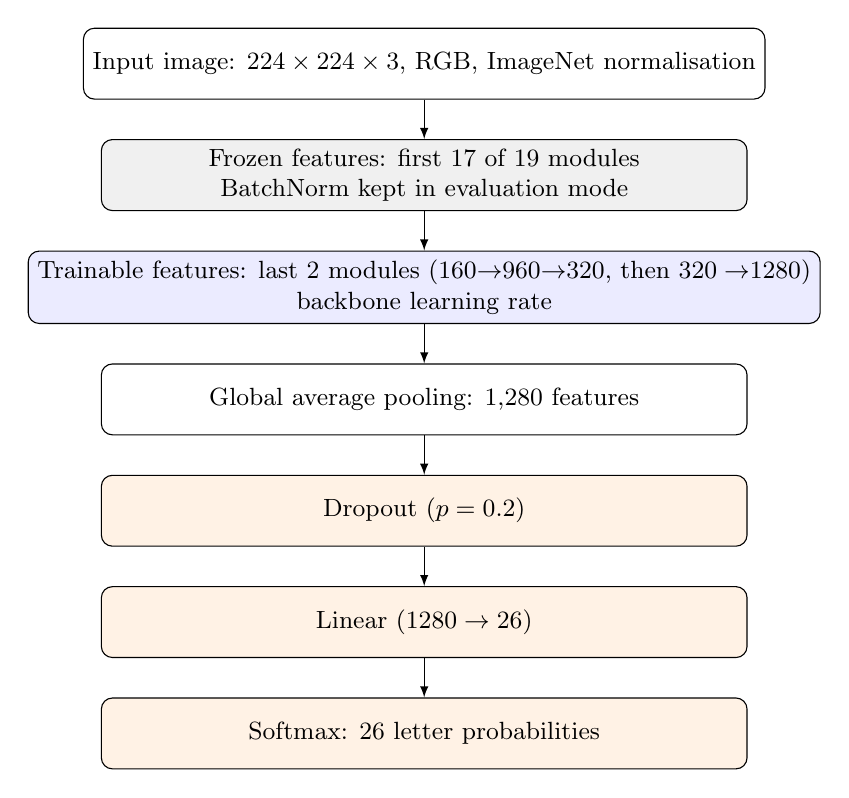
\begin{tikzpicture}[
  node distance=5mm,
  box/.style={draw, rounded corners, align=center, font=\small,
              minimum width=8.2cm, minimum height=9mm},
  frozen/.style={box, fill=gray!12},
  trainable/.style={box, fill=blue!8},
  head/.style={box, fill=orange!10},
  >=latex
]
\node[box] (input) {Input image: $224\times224\times3$, RGB, ImageNet normalisation};
\node[frozen, below=of input] (frozen) {Frozen features: first 17 of 19 modules\\BatchNorm kept in evaluation mode};
\node[trainable, below=of frozen] (tuned) {Trainable features: last 2 modules (160$\to$960$\to$320, then $320\to$1280)\\backbone learning rate};
\node[box, below=of tuned] (pool) {Global average pooling: 1{,}280 features};
\node[head, below=of pool] (dropout) {Dropout ($p=0.2$)};
\node[head, below=of dropout] (linear) {Linear ($1280\to26$)};
\node[head, below=of linear] (softmax) {Softmax: 26 letter probabilities};
\draw[->] (input) -- (frozen);
\draw[->] (frozen) -- (tuned);
\draw[->] (tuned) -- (pool);
\draw[->] (pool) -- (dropout);
\draw[->] (dropout) -- (linear);
\draw[->] (linear) -- (softmax);
\end{tikzpicture}
\caption{Data flow of the MobileNetV2 classifier. The grey block is frozen, the blue block is fine-tuned, and the orange blocks form the new classifier head. The diagram shows the default \texttt{unfreeze\_blocks: 2}; a value of 0 freezes the whole blue block and a larger value unfreezes more modules.}
\label{fig:cnn-architecture}
\end{figure}

\section{CNN Hyperparameter Search}
\label{sec:cnn-hyperparameters}

\subsection{Search Space}

The tuning grid is stored in \texttt{configs/cnn.yaml} and read by \texttt{python -m signbridge.tune\_cnn}. Five hyperparameters are varied: the head learning rate, the batch size, the dropout probability, the AdamW weight decay and the number of unfrozen feature modules. The grid in Table~\ref{tab:cnn-search-space} contains $2^5=32$ combinations. Training is capped at 12 trials, and each trial runs for 3 epochs. The 12 trials are a seeded random sample, not the first 12 rows of the grid: \texttt{random.Random} with the config seed (42) shuffles all 32 combinations, duplicate combinations are removed, and the search walks that shuffled order from the start and runs at most 12 trials. A position whose parameter set and seed are already in the trials file is skipped, so an interrupted search fills the remaining budget in the same order instead of starting a new search. Early stopping is configured with patience 3, so it does not trigger inside a 3-epoch trial. These short trials are intended to rank configurations, not to produce the final model.

\begin{table}[htbp]
\centering
\caption{CNN hyperparameter search space in \texttt{configs/cnn.yaml}.}
\label{tab:cnn-search-space}
\begin{tabular}{lll}
\toprule
Hyperparameter & Values & Role \\
\midrule
Head learning rate & $3\times10^{-4}$, $1\times10^{-3}$ & step size for the new classifier \\
Batch size & 32, 64 & images per optimisation step \\
Dropout & 0.2, 0.4 & regularisation before the linear layer \\
Weight decay & $1\times10^{-4}$, $1\times10^{-3}$ & AdamW regularisation \\
Unfrozen blocks & 0, 2 & last feature modules trained \\
\midrule
Trials & at most 12 of 32 & seeded random sample, hard cap \\
Epochs per trial & 3 & short ranking runs \\
\bottomrule
\end{tabular}
\end{table}

The remaining settings are fixed during tuning: 26 classes, ImageNet-pretrained MobileNetV2, $224\times224$ input, cross-entropy with label smoothing 0.1, AdamW with a backbone learning rate multiplier of 0.1, cosine annealing, early-stopping patience 3 and seed 42. The final run uses the same configuration with 10 to 15 epochs and early stopping.

\subsection{Selection Rule}

A trial is ranked by its best validation macro-F1. Ties are broken in favour of the trial with fewer trainable parameters, because a smaller model is cheaper to train and to run and is less likely to overfit. The rule is written in the docstring of \texttt{tune\_cnn.py} and in \texttt{DECISIONS.md}. The test split is never read during tuning. Each trial appends one row to \texttt{reports/tuning/cnn\_trials.csv}; a parameter set and seed that already appear in that file are skipped, so an interrupted search can be resumed without repeating work.

\subsection{Trial Results}

\IfFileExists{../../reports/tuning/cnn_trials_table.tex}{%
  \begin{table}[htbp]
  \centering
  \caption{Tuning trials for the CNN, ordered as recorded. The table is generated from \texttt{reports/tuning/cnn\_trials.csv} by \texttt{tools/trials\_to\_tex.py}.}
  \label{tab:cnn-trials}
  \resizebox{\linewidth}{!}{\begin{tabular}{lrrrrrrrrr}
\hline
run\_name & lr & batch\_size & dropout & weight\_decay & unfreeze\_blocks & best\_val\_macro\_f1 & val\_accuracy & epochs\_run & seconds \\
\hline
trial\_000 & 0.001 & 64 & 0.2 & 0.001 & 0 & 0.8065300626970106 & 0.8108974358974359 & 3 & 132.15 \\
trial\_001 & 0.0003 & 32 & 0.4 & 0.0001 & 2 & 0.8794509384109741 & 0.8801282051282051 & 3 & 125.61 \\
trial\_002 & 0.0003 & 64 & 0.2 & 0.001 & 0 & 0.6753639935073358 & 0.6820512820512821 & 3 & 129.19 \\
trial\_003 & 0.0003 & 64 & 0.4 & 0.001 & 2 & 0.8430798718360818 & 0.8442307692307692 & 3 & 132.34 \\
trial\_004 & 0.001 & 64 & 0.2 & 0.0001 & 2 & 0.9225361978376546 & 0.9224358974358975 & 3 & 131.39 \\
trial\_005 & 0.0003 & 64 & 0.2 & 0.001 & 2 & 0.8527992548457175 & 0.8538461538461538 & 3 & 131.39 \\
trial\_006 & 0.001 & 32 & 0.4 & 0.001 & 0 & 0.8288342444338248 & 0.8314102564102565 & 3 & 126.31 \\
trial\_007 & 0.0003 & 32 & 0.4 & 0.001 & 0 & 0.7260288440272608 & 0.732051282051282 & 3 & 124.31 \\
trial\_008 & 0.001 & 32 & 0.2 & 0.001 & 2 & 0.9437027962531004 & 0.9442307692307692 & 3 & 127.6 \\
trial\_009 & 0.0003 & 64 & 0.4 & 0.0001 & 0 & 0.6644214014818777 & 0.6705128205128205 & 3 & 128.42 \\
trial\_010 & 0.001 & 32 & 0.2 & 0.0001 & 0 & 0.8364909320199915 & 0.8384615384615385 & 3 & 123.65 \\
trial\_011 & 0.0003 & 64 & 0.2 & 0.0001 & 2 & 0.8527992548457175 & 0.8538461538461538 & 3 & 132.25 \\
\hline
\end{tabular}
}
  \end{table}
}{%
  \todobox{The CNN trial table is missing. It will be generated from \texttt{reports/tuning/cnn\_trials.csv} by \texttt{tools/trials\_to\_tex.py} after the real tuning runs on the shared split.}
}

\todobox{Justification of the final chosen hyperparameters, to be written after the real tuning runs and after the best trial is known.}

\section{Landmark Models}
\label{sec:landmark-models}

\subsection{Framework and Pipeline}

The landmark branch classifies a hand image in two stages. First, the MediaPipe hand landmarker finds one hand and returns 21 landmarks, each with $x$, $y$ and $z$ coordinates (Section~\ref{sec:feature-results}). The coordinates are normalised relative to the wrist and flattened into a vector of $21\times3=63$ values. Second, a classifier maps this vector to a probability for each of the 26 letters, in the class order of \texttt{data/processed/label\_map.json}. Three classifier families are trained on the same vectors: a support vector machine and a random forest from scikit-learn, and a multilayer perceptron (MLP) written in PyTorch. The code is in \texttt{src/signbridge/models/landmark\_models.py} and the training command is \texttt{src/signbridge/train\_landmark.py}.

\begin{figure}[htbp]
\centering
\resizebox{\linewidth}{!}{%
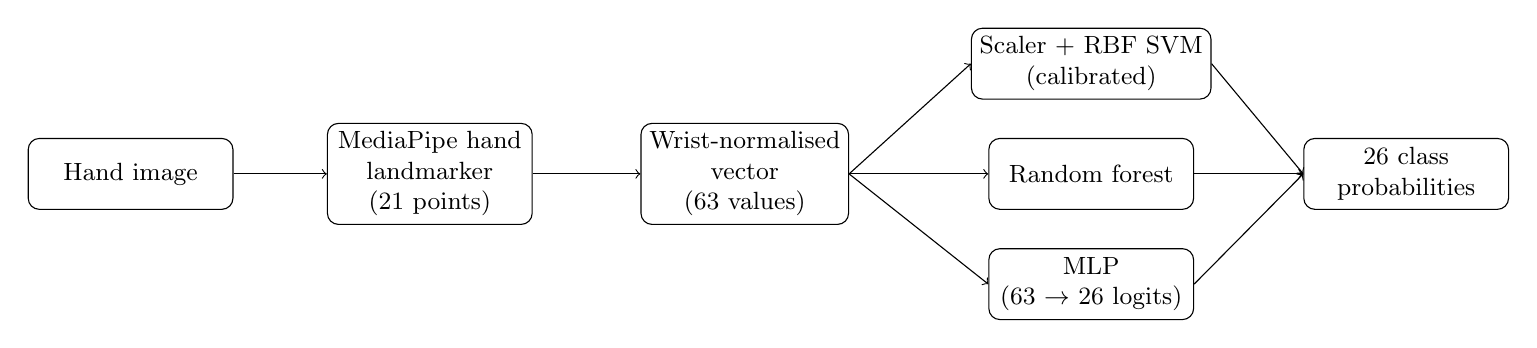
\begin{tikzpicture}[box/.style={draw, rounded corners, align=center, minimum width=2.6cm, minimum height=0.9cm, inner sep=3pt, font=\small}]
  \node[box] (img) at (0,0) {Hand image};
  \node[box] (mp) at (3.8,0) {MediaPipe hand\\landmarker\\(21 points)};
  \node[box] (norm) at (7.8,0) {Wrist-normalised\\vector\\(63 values)};
  \node[box] (svm) at (12.2,1.4) {Scaler + RBF SVM\\(calibrated)};
  \node[box] (rf) at (12.2,0) {Random forest};
  \node[box] (mlp) at (12.2,-1.4) {MLP\\(63 $\to$ 26 logits)};
  \node[box] (out) at (16.2,0) {26 class\\probabilities};
  \draw[->] (img) -- (mp);
  \draw[->] (mp) -- (norm);
  \draw[->] (norm.east) -- (svm.west);
  \draw[->] (norm.east) -- (rf.west);
  \draw[->] (norm.east) -- (mlp.west);
  \draw[->] (svm.east) -- (out.west);
  \draw[->] (rf.east) -- (out.west);
  \draw[->] (mlp.east) -- (out.west);
\end{tikzpicture}%
}
\caption{The landmark pipeline. Images in which no hand is found stop after the landmarker and receive no prediction.}
\label{fig:landmark-pipeline}
\end{figure}

\subsection{Classical Baselines}

\textbf{Support vector machine.} The SVM is a pipeline of a \texttt{StandardScaler} and an RBF-kernel \texttt{SVC}, with the regularisation $C$ and the kernel width $\gamma$ as hyperparameters. The AUC-ROC metric needs class probabilities, which an \texttt{SVC} does not give by default. The earlier plan was to switch on the \texttt{probability=True} option. In scikit-learn 1.9 that option is deprecated and planned for removal in version 1.11, so the \texttt{SVC} is wrapped in \texttt{CalibratedClassifierCV} with sigmoid calibration, 5 folds and \texttt{ensemble=False}. The calibrator is fitted on cross-validated decision values and the \texttt{SVC} is then refitted once on all training data, so every SVM fit trains the \texttt{SVC} six times. The output is an $n\times26$ matrix whose rows sum to 1, which is checked by a unit test. The calibration needs at least 5 training images per class.

\textbf{Random forest.} The forest is a scikit-learn \texttt{RandomForestClassifier} with the number of trees and the maximum depth as hyperparameters. Tree models do not depend on feature scale, so no scaler is used.

\subsection{Multilayer Perceptron}

The MLP takes the 63 landmark values after standardisation. The mean and standard deviation are computed on the training split only. Each hidden block is a linear layer, a ReLU activation and dropout, and the output layer is a linear layer with 26 logits (Table~\ref{tab:landmark-mlp-layers}). The number of hidden layers is fixed at two, while the hidden width and the dropout probability are tuned (Section~\ref{sec:landmark-hyperparameters}). With the settings of the best search trial (width 256) the network has $63\cdot256+256 + 256\cdot256+256 + 256\cdot26+26 = 88{,}858$ trainable parameters, computed from the layer sizes.

\begin{table}[htbp]
\centering
\caption{Layers of the landmark MLP. $h$ is the hidden width and $p$ the dropout probability.}
\label{tab:landmark-mlp-layers}
\begin{tabular}{lll}
\toprule
Layer & Output size & Note \\
\midrule
Input & 63 & standardised landmark values \\
Linear, ReLU, Dropout($p$) & $h$ & repeated for each hidden layer \\
Linear & 26 & logits, one per letter \\
\bottomrule
\end{tabular}
\end{table}

\textbf{Loss.} The loss is \texttt{CrossEntropyLoss}. It combines a log-softmax with the negative log-likelihood, so the network outputs raw logits and the softmax is applied only when probabilities are needed. Cross-entropy is the standard choice for a single-label problem with 26 mutually exclusive classes.

\textbf{Optimiser.} Training uses AdamW, which applies weight decay separately from the gradient step. Learning rate, weight decay and batch size are tuned. Batches are shuffled with a seeded generator.

\textbf{Early stopping.} Training runs for at most 100 epochs. After each epoch the model is scored on the validation split, with dropout switched off. If the validation macro-F1 does not improve for 10 epochs, training stops and the weights of the best epoch are restored. Loss and accuracy of both splits are written for every epoch to \texttt{reports/tuning/mlp\_history.csv}, which gives the learning curves.

\subsection{Training Procedure and Use of the Splits}

One command trains the models and writes the predictions: \texttt{python -m signbridge.train\_landmark}. The seed comes from \texttt{configs/data.yaml} and is logged. The shared group-aware split (Section~\ref{sec:validation}) has 280 training, 60 validation and 60 test images per letter, before images without a detected hand are removed. The validation split is used for early stopping and for all hyperparameter selection. The test split is read only by the final run (\texttt{--final --evaluate-test}), which was made once, after the chosen settings had been committed to \texttt{configs/landmark.yaml}. The family with the highest validation macro-F1 in the final run is treated as the landmark model, and its prediction files are copied to \texttt{reports/predictions/landmark\_val.npz} and \texttt{landmark\_test.npz}. The files of the other families are kept next to them. No cross-validation was run.

\subsection{Limitation: Images Without a Detected Hand}

A landmark model can only predict for images in which MediaPipe finds a hand. Images without a detection are not counted as errors; they are missing from the prediction files, so landmark scores describe the detected images only and cannot be read as accuracy on all images. We kept the default detection confidence of 0.5, because a wrong landmark vector is worse than a missing one.

The extraction ran once on all 10{,}400 images of the shared split. No image was unreadable and no landmark vector contained a non-finite value. A hand was found in 7{,}660 images (73.7\%), with similar rates in the three splits (Table~\ref{tab:landmark-detection}). The 20-image check of Section~\ref{sec:feature-results} (15 of 20, or 75\%) was close to this overall rate.

\begin{table}[htbp]
\centering
\caption{Images with a detected hand in each split of the shared split file.}
\label{tab:landmark-detection}
\begin{tabular}{lrrr}
\toprule
Split & Images & Hand found & Rate \\
\midrule
Train & 7{,}280 & 5{,}475 & 75.2\% \\
Validation & 1{,}560 & 1{,}095 & 70.2\% \\
Test & 1{,}560 & 1{,}090 & 69.9\% \\
\midrule
All & 10{,}400 & 7{,}660 & 73.7\% \\
\bottomrule
\end{tabular}
\end{table}

The rate differs strongly between letters. Of the 400 images per letter, a hand was found in only 130 images of N (32.5\%), 193 of M (48.2\%), 242 of A (60.5\%), 259 of P (64.8\%), 260 of C (65.0\%) and 262 of Q (65.5\%). The highest rates are F (382 images, 95.5\%), K (348, 87.0\%) and R (337, 84.2\%). The lowest letters include the closed-hand signs A, M and N. In the 20-image check, three of the five missed images showed closed or curled fingers and two showed fingers pointing downwards. We did not inspect the missed images of the full run, so we do not claim a cause for the full set.

Only the detected images are used: 5{,}475 for training, 1{,}095 for validation and 1{,}090 for testing. Because the detection rate depends on the letter, the landmark test set is no longer balanced: the number of test images per letter ranges from 20 (A) to 57 (F), out of 60 in the split.

\subsection{Final Scores}

The final run trained the three families with the committed settings and wrote the validation and test predictions in one command, run once. On validation the SVM had the highest macro-F1 (0.9683), ahead of the MLP (0.9678) and the forest (0.9495), so the SVM is the landmark model (Section~\ref{sec:landmark-hyperparameters}). Table~\ref{tab:landmark-scores} shows its scores, computed with the shared evaluation code on the detected images only.

\begin{table}[htbp]
\centering
\caption{Scores of the landmark model (calibrated SVM) on the detected images.}
\label{tab:landmark-scores}
\begin{tabular}{lrrrr}
\toprule
Split & Images & Accuracy & Macro-F1 & Macro AUC-ROC \\
\midrule
Validation & 1{,}095 & 0.9753 & 0.9683 & 0.9940 \\
Test & 1{,}090 & 0.9688 & 0.9660 & 0.9951 \\
\bottomrule
\end{tabular}
\end{table}

Per letter, the SVM is weakest on the test split for M (F1 0.857, 22 test images), N (0.889, 24 images) and S (0.916, 55 images), followed by I (0.938) and J (0.947). The letters B, D, K, L and U have an F1 of 1.000. M and N are also among the letters with the lowest detection rates, so their scores rest on few images and are noisy. The confused letter pairs are analysed in the error analysis section.

On the same 1{,}090 test images the CNN reached accuracy 0.9780, macro-F1 0.9789 and macro AUC-ROC 0.9998. The CNN is therefore ahead of the landmark model on these images by 0.0092 in accuracy (about ten images) and by 0.0129 in macro-F1.

These scores are optimistic and are not an estimate of accuracy on new signers. As Section~\ref{sec:limitations} reports, 70.0\% of the test images and 73.4\% of the validation images have a training image of the same class within 8 bits of the difference hash. Near-identical images in training and test make every score in this report higher than it would be on new people. That check covers all test images; we did not repeat it for the 1{,}090 detected images that the landmark model uses.

\subsection{Learning Curves}

Figure~\ref{fig:landmark-mlp-curves} shows the loss and accuracy of the final MLP run, which uses the settings of the best search trial, for every epoch. Training ran for 32 epochs. At epoch 1 the training accuracy was 0.7191 and the validation accuracy 0.8612. The best validation macro-F1 (0.9678, validation accuracy 0.9717) was reached at epoch 22, where the training accuracy was 0.9799. After 10 epochs without improvement training stopped at epoch 32, and the weights of epoch 22 were restored.

\IfFileExists{\figdir landmark_mlp_curves.png}{%
  \begin{figure}[htbp]
  \centering
  \includegraphics[width=0.95\linewidth]{\figdir landmark_mlp_curves.png}
  \caption{Loss and accuracy per epoch of the final landmark MLP run, for the training and validation splits.}
  \label{fig:landmark-mlp-curves}
  \end{figure}
}{%
  \todobox{Missing figure \texttt{reports/figures/landmark\_mlp\_curves.png}. Make it with \texttt{python -m signbridge.plot\_landmark\_curves}.}
}

The validation loss was 0.2245 at epoch 22, lowest at epoch 24, and 0.3106 at epoch 32. Over the same epochs the training loss stayed between 0.055 and 0.064, and the validation macro-F1 fell to 0.9553. This points to mild overfitting after about epoch 22 to 24, which is why the best weights are restored. The gap between training accuracy (0.9799) and validation accuracy (0.9717) at epoch 22 is about 0.8 percentage points. The training loss is averaged over the epoch with dropout active, and the validation loss is computed with dropout off, so the two losses are not directly comparable.
\section{Landmark Hyperparameter Search}
\label{sec:landmark-hyperparameters}

\subsection{Search Space}

The tuning grid is stored in \texttt{configs/landmark.yaml} and read by \texttt{python -m signbridge.tune\_landmark}. The SVM and the random forest use their full grids: $4\times4=16$ SVM trials and $3\times3=9$ forest trials. The MLP grid has five hyperparameters with three values each, $3^5=243$ combinations, which is too many to train. A seeded random sample of 20 combinations (8.2\%) was run instead (Table~\ref{tab:landmark-search-space}), so 45 trials were run in total. Each trial was run once with seed 42 and appended one row to \texttt{reports/tuning/landmark\_trials.csv}, which has its own columns for the SVM, forest and MLP parameters. A trial that is already in the file is skipped, so an interrupted search can be resumed. The first SVM trial was run alone to time it, and the full search reused its row. Every trial is trained on the training split and scored on the validation split. The file has no test column, and the test split is never read during tuning.

\begin{table}[htbp]
\centering
\caption{Landmark hyperparameter search space in \texttt{configs/landmark.yaml}.}
\label{tab:landmark-search-space}
\begin{tabular}{lll}
\toprule
Model & Hyperparameter & Values \\
\midrule
SVM & $C$ & 0.1, 1, 10, 100 \\
SVM & $\gamma$ & scale, 0.01, 0.1, 1 \\
Random forest & Number of trees & 100, 300, 500 \\
Random forest & Maximum depth & none, 10, 20 \\
MLP & Learning rate & $3\times10^{-4}$, $1\times10^{-3}$, $3\times10^{-3}$ \\
MLP & Batch size & 32, 64, 128 \\
MLP & Dropout & 0.1, 0.3, 0.5 \\
MLP & Hidden width & 64, 128, 256 \\
MLP & Weight decay & 0, $1\times10^{-4}$, $1\times10^{-3}$ \\
\midrule
Trials & SVM / forest / MLP & 16 / 9 / 20 (seeded sample of 243) \\
\bottomrule
\end{tabular}
\end{table}

The remaining settings are fixed during tuning: two hidden layers, at most 100 epochs, early-stopping patience 10, AdamW, 63 inputs, 26 classes and seed 42. The search was fast: the per-trial times add up to 361 s, about 6 minutes. An SVM trial took 1.8 to 12.4 s, a forest trial 0.5 to 2.8 s and an MLP trial 4.6 to 22.6 s, so the MLP trials took most of the time (255 s). No grid had to be reduced.

\subsection{Selection Rule}

Within each model family, the trial with the highest validation macro-F1 wins. Macro-F1 is used because it weights all 26 letters equally and shows letters that fail, even though the classes are balanced in the split. If two trials of a family have exactly the same validation macro-F1, the one recorded first in the trials file is kept; there is no further tie-break. The winning settings of the three families were written to \texttt{configs/landmark.yaml} in one commit that names the winning trials, before the final training run. The three winners are then retrained in the final run, and the family with the highest validation macro-F1 in that run is treated as the landmark model.

\subsection{Trial Results}

Tables~\ref{tab:landmark-svm-trials}, \ref{tab:landmark-forest-trials} and \ref{tab:landmark-mlp-trials} list every trial, with the numbers copied from \texttt{reports/tuning/\allowbreak landmark\_trials.csv}.

\begin{table}[htbp]
\centering
\caption{Validation macro-F1 of the 16 SVM trials (rows: $C$, columns: $\gamma$). The winner, svm-14, is marked with an asterisk.}
\label{tab:landmark-svm-trials}
\begin{tabular}{lrrrr}
\toprule
$C$ & $\gamma$ = scale & $\gamma$ = 0.01 & $\gamma$ = 0.1 & $\gamma$ = 1 \\
\midrule
0.1 & 0.8161 & 0.7819 & 0.8650 & 0.5822 \\
1 & 0.9475 & 0.9340 & 0.9439 & 0.8278 \\
10 & 0.9669 & 0.9650 & 0.9486 & 0.8285 \\
100 & 0.9648 & 0.9683$^{*}$ & 0.9478 & 0.8285 \\
\bottomrule
\end{tabular}
\end{table}

\begin{table}[htbp]
\centering
\caption{Validation macro-F1 of the 9 forest trials (rows: number of trees, columns: maximum depth). The winner, forest-06, is marked with an asterisk.}
\label{tab:landmark-forest-trials}
\begin{tabular}{lrrr}
\toprule
Trees & Depth none & Depth 10 & Depth 20 \\
\midrule
100 & 0.9419 & 0.9324 & 0.9411 \\
300 & 0.9487 & 0.9290 & 0.9495$^{*}$ \\
500 & 0.9479 & 0.9314 & 0.9488 \\
\bottomrule
\end{tabular}
\end{table}

\begin{table}[htbp]
\centering
\small
\caption{The 20 MLP trials. LR is the learning rate and WD the weight decay. The winner, mlp-16, is marked with an asterisk.}
\label{tab:landmark-mlp-trials}
\begin{tabular}{lrrrrrrr}
\toprule
Trial & LR & Batch & Dropout & Width & WD & Macro-F1 & Accuracy \\
\midrule
mlp-01 & 0.0003 & 32 & 0.5 & 64 & 0.0001 & 0.9283 & 0.9379 \\
mlp-02 & 0.0003 & 32 & 0.5 & 128 & 0 & 0.9556 & 0.9607 \\
mlp-03 & 0.0003 & 64 & 0.1 & 128 & 0 & 0.9674 & 0.9708 \\
mlp-04 & 0.0003 & 64 & 0.5 & 64 & 0.0001 & 0.9350 & 0.9452 \\
mlp-05 & 0.001 & 32 & 0.3 & 256 & 0.001 & 0.9644 & 0.9689 \\
mlp-06 & 0.001 & 32 & 0.5 & 64 & 0 & 0.9481 & 0.9562 \\
mlp-07 & 0.001 & 64 & 0.1 & 64 & 0.0001 & 0.9598 & 0.9635 \\
mlp-08 & 0.001 & 64 & 0.3 & 256 & 0 & 0.9651 & 0.9689 \\
mlp-09 & 0.001 & 128 & 0.3 & 128 & 0 & 0.9701 & 0.9735 \\
mlp-10 & 0.001 & 128 & 0.5 & 256 & 0.001 & 0.9610 & 0.9671 \\
mlp-11 & 0.003 & 32 & 0.1 & 256 & 0.001 & 0.9695 & 0.9735 \\
mlp-12 & 0.003 & 32 & 0.3 & 64 & 0.001 & 0.9622 & 0.9689 \\
mlp-13 & 0.003 & 32 & 0.3 & 128 & 0 & 0.9609 & 0.9680 \\
mlp-14 & 0.003 & 32 & 0.5 & 64 & 0 & 0.9411 & 0.9525 \\
mlp-15 & 0.003 & 32 & 0.5 & 256 & 0.0001 & 0.9548 & 0.9635 \\
mlp-16$^{*}$ & 0.003 & 64 & 0.1 & 256 & 0.0001 & 0.9716 & 0.9753 \\
mlp-17 & 0.003 & 64 & 0.3 & 128 & 0.001 & 0.9651 & 0.9699 \\
mlp-18 & 0.003 & 128 & 0.3 & 128 & 0.0001 & 0.9661 & 0.9717 \\
mlp-19 & 0.003 & 128 & 0.5 & 64 & 0 & 0.9358 & 0.9470 \\
mlp-20 & 0.003 & 128 & 0.5 & 128 & 0.001 & 0.9615 & 0.9680 \\
\bottomrule
\end{tabular}
\end{table}

\subsection{Winners and Justification}

Table~\ref{tab:landmark-winners} shows the winner of each family and its score in the final run, in which the winners were retrained once with the same settings.

\begin{table}[htbp]
\centering
\caption{Winning trial per family. Search scores are validation scores from the trials file; the last column is the validation macro-F1 of the retrained model in the final run.}
\label{tab:landmark-winners}
\resizebox{\linewidth}{!}{%
\begin{tabular}{lp{6.3cm}rrr}
\toprule
Family & Winning trial and settings & Search macro-F1 & Search accuracy & Final-run macro-F1 \\
\midrule
SVM & svm-14: $C=100$, $\gamma=0.01$ & 0.9683 & 0.9753 & 0.9683 \\
Random forest & forest-06: 300 trees, maximum depth 20 & 0.9495 & 0.9543 & 0.9495 \\
MLP & mlp-16: learning rate 0.003, batch size 64, dropout 0.1, hidden width 256, weight decay 0.0001 & 0.9716 & 0.9753 & 0.9678 \\
\bottomrule
\end{tabular}%
}
\end{table}

\textbf{SVM.} The macro-F1 over the 16 trials ranges from 0.5822 to 0.9683. For every $C$, $\gamma=1$ gave the lowest score of its row (0.5822 to 0.8285), and with $C=0.1$ no $\gamma$ reached 0.87. The best values of $\gamma$ are 0.01 and ``scale'', which is about $1/63\approx0.016$ for standardised inputs, and $\gamma=0.1$ is lower again (0.9478 to 0.9486 for $C\geq10$). The winner has the largest $C$ of the grid, so larger values were not tested. The last step in $C$ (10 to 100) changed the macro-F1 by $+0.0033$ at $\gamma=0.01$ and by $-0.0021$ at $\gamma=$ scale, so a larger $C$ is unlikely to change the picture much, but we did not test it. The two next-best trials, svm-09 (0.9669) and svm-10 (0.9650), are within 0.0033; the validation accuracy of svm-14 is 0.9753 and that of svm-09 is 0.9726, a difference of about three images out of 1{,}095.

\textbf{Random forest.} The macro-F1 ranges from 0.9290 to 0.9495. A maximum depth of 10 was the worst depth for every number of trees (0.9290 to 0.9324) and cost 0.009 to 0.021 macro-F1 compared with depth 20. Depth 20 and no depth limit are close (within 0.0008 at every number of trees). More trees helped from 100 to 300 (0.9411 to 0.9495 at depth 20) but not from 300 to 500 (0.9488). The forest is the weakest family: its best trial is 0.0188 below the best SVM trial and 0.0221 below the best MLP trial.

\textbf{MLP.} The macro-F1 ranges from 0.9283 to 0.9716. The best trial has the lowest dropout (0.1), the largest width (256) and the highest learning rate (0.003) of the grid. Very different settings score almost the same: mlp-09 (learning rate 0.001, batch size 128, dropout 0.3, width 128) reaches 0.9701 and mlp-11 reaches 0.9695. The five lowest trials (0.9283 to 0.9481) are exactly the five that combine dropout 0.5 with width 64. Only 20 of 243 combinations were tried, so mlp-16 is the best of a random sample and not of the grid, and several of its values lie at the edge of the grid.

\textbf{Which family is the landmark model.} In the search the best MLP (0.9716) was ahead of the best SVM (0.9683) by 0.0033. In the final run the retrained SVM and forest reproduce their search scores exactly (0.9683 and 0.9495), but the retrained MLP scored 0.9678, which is 0.0038 below its search score and 0.0005 below the SVM. By the selection rule the SVM is therefore the landmark model; the search scores alone would have chosen the MLP. We did not find the cause of the MLP difference and did not run other seeds. The initial weights are created before the training function sets its seed, so they may depend on earlier work in the same process, but we did not test whether this explains it. Because the same MLP settings changed by 0.0038 between two runs, and one validation image is 0.09 percentage points of accuracy, we do not claim that the SVM is better than the MLP: the two are tied within the variation we measured. The forest is clearly behind both.

\textbf{Limits of the search.} Each trial used one seed, the MLP search covers 8.2\% of its grid, and the winners of the SVM and MLP have values at the edge of their grids. The search selects settings on 1{,}095 validation images from the detected images only, so small differences between the top trials should not be read as a ranking.
\section{Metrics}
\label{sec:metrics}

The function \texttt{evaluate} in \texttt{src/signbridge/evaluation/metrics.py} takes the true class indices, the predicted probabilities (one row per image, one column per letter) and the class names. The predicted letter is the class with the highest probability. It returns the metrics below, which are computed with scikit-learn and saved as JSON, a per-class CSV and a confusion matrix figure.

\subsection{Definitions}

For one class, let TP, FP and FN be the numbers of true positives, false positives and false negatives.
\begin{align*}
  \text{precision} &= \frac{TP}{TP + FP}, &
  \text{recall} &= \frac{TP}{TP + FN}, &
  F_1 &= \frac{2 \cdot \text{precision} \cdot \text{recall}}{\text{precision} + \text{recall}}.
\end{align*}
Accuracy is the share of images whose predicted letter is correct. Macro precision, recall and $F_1$ are the unweighted means of the 26 per-class values. A class that is never predicted has precision 0 by convention. The confusion matrix has one row per true letter and one column per predicted letter.

\textbf{AUC-ROC.} The multiclass AUC-ROC is computed one-vs-rest. For each letter, the images of that letter are the positives and all other images are the negatives, and the probability of that letter is the score. The area under the ROC curve is the chance that a random image of the letter gets a higher score than a random image of another letter. The 26 areas are averaged without weights (macro average). The probabilities of each row must sum to 1; the function checks this and stops with an error otherwise. The AUC of a letter is undefined if that letter does not occur in the data, so the function also stops with an error in that case.

\subsection{Why these Metrics}
\begin{itemize}
  \item \textbf{Accuracy} is the simplest summary. It is easy to read here because the data is balanced: every class has 60 test images (Section~\ref{sec:validation}). On such a test set the macro recall equals the accuracy.
  \item \textbf{Macro and per-class precision, recall and $F_1$} are used to show which letters fail, not to correct for class imbalance, because there is none. Precision tells how often a predicted letter is right, recall how many images of a letter are found, and $F_1$ combines both. Several ASL letters are similar closed-fist shapes, so the per-class values can show which pairs a model confuses.
  \item \textbf{Macro AUC-ROC} measures how well the probabilities rank the correct letter above the others, independently of the decision rule. It can show that one model has better-calibrated scores even when two models have the same accuracy.
  \item \textbf{The confusion matrix} shows which letters are mistaken for which, and is the basis of the error analysis in Section~\ref{sec:error-analysis}.
\end{itemize}

\subsection{Limits}
\begin{itemize}
  \item The landmark model can only run on images where MediaPipe finds a hand, so both models are also compared on that common subset of the test set. There the classes are no longer perfectly balanced, and the macro recall can differ from the accuracy.
  \item With 60 test images per class, each per-class value is coarse: one image is 1.7 percentage points of recall. The per-class numbers should be read as indications, not as exact values.
  \item The metrics are computed on one split of the ASL baseline and do not measure how the models will do on PSL.
\end{itemize}

\section{Results}
\label{sec:results}

All results in this section describe the American Sign Language (ASL) baseline, not Pakistan Sign Language, and were computed with our own evaluation code (\texttt{src/signbridge/evaluation/}) from the prediction files in \texttt{reports/predictions/}. The metrics are defined in Section~\ref{sec:metrics}. The test split was used once, after the hyperparameters were frozen (Section~\ref{sec:validation}).

\subsection{CNN}

Table~\ref{tab:cnn-results} shows the validation and test metrics of the final CNN. Both splits hold 1{,}560 images, 60 per letter, so accuracy and macro recall are equal. The CNN made 49 mistakes on the validation split and 32 on the test split.

\begin{table}[htbp]
  \centering
  \caption{Metrics of the final CNN on the validation and test splits (ASL baseline). Source: \texttt{reports/metrics/cnn\_val\_metrics.json} and \texttt{cnn\_test\_metrics.json}. Macro values average the 26 letters.}
  \label{tab:cnn-results}
  \begin{tabular}{lcc}
    \toprule
    Metric & Validation & Test \\
    \midrule
    Images & 1{,}560 & 1{,}560 \\
    Mistakes & 49 & 32 \\
    Accuracy & 0.9686 & 0.9795 \\
    Macro precision & 0.9694 & 0.9798 \\
    Macro recall & 0.9686 & 0.9795 \\
    Macro F1 & 0.9686 & 0.9795 \\
    Macro AUC-ROC (one-vs-rest) & 0.9996 & 0.9998 \\
    \bottomrule
  \end{tabular}
\end{table}

The test scores are 1.1 points higher than the validation scores. This is about 17 images out of 1{,}560, and we have no evidence that the difference means more than chance, since the two splits contain different images and, as Table~\ref{tab:cnn-results} shows, each letter has only 60 of them. The training and validation curves of the final run are in Figures~\ref{fig:cnn-loss} and~\ref{fig:cnn-accuracy}. The most confused letters and the weakest letters are in Section~\ref{sec:error-analysis}, and the scores by brightness, blur and hand detection are in Section~\ref{sec:bias-check}.

The two figures below show the nine epochs of the final CNN run. Training loss falls in every epoch, from 1.549 to 0.766, and training accuracy rises from 0.728 to 0.992. Validation loss falls from 1.086 to a minimum of 0.810 at epoch 9, but validation accuracy and macro-F1 peak at epoch 6, both at 0.9686, and are lower afterwards. The widening gap between training and validation accuracy after epoch 6 is the overfitting that early stopping is meant to catch, and the checkpoint from epoch 6 was kept. The run stopped after epoch 9 because the validation macro-F1 had not improved for three consecutive epochs. How far these scores can be trusted is discussed in Section~\ref{sec:read-scores}.

\safefigure{cnn_loss_curve.png}{Training and validation loss per epoch for the final CNN run, from \texttt{reports/training/cnn\_history.csv}.}{fig:cnn-loss}

\safefigure{cnn_accuracy_curve.png}{Training and validation accuracy per epoch for the final CNN run, from \texttt{reports/training/cnn\_history.csv}.}{fig:cnn-accuracy}

\subsection{How to Read These Scores}
\label{sec:read-scores}

The scores are close to 100\%, and they should not be read as the accuracy the system would have on new people. The ASL images are frames from short recordings, and our split removes only the nearest duplicates, so many validation and test images have a very similar training image of the same letter (Section~\ref{sec:limitations}): 20.3\% of the test images have a same-class training image within 4 bits of the image hash, 47.2\% within 6 bits and 70.0\% within 8 bits. The dataset also has no signer identifiers, so we cannot tell whether the same people appear in training and test. For both reasons the scores are optimistic, and we do not call the model robust. A fair estimate for new signers needs a person-wise split on data with signer labels, such as the planned PSL collection (Section~\ref{sec:data-collection}).

\subsection{CNN Compared with the Landmark Models}

The landmark models (Section~\ref{sec:landmark-models}) classify the 21 hand landmarks that MediaPipe finds in an image, so they can only give an answer for images where a hand was detected. This is 1{,}090 of the 1{,}560 test images (69.9\%). A comparison on all test images would favour the CNN, which answers every image, so Table~\ref{tab:common-set} compares all four models on the same 1{,}090 images (the common set), computed with \texttt{run\_metrics} and its \texttt{--restrict-to} option on the files in \texttt{reports/predictions/}. For reference, the CNN scores 0.9795 accuracy on all 1{,}560 test images (Table~\ref{tab:cnn-results}).

\begin{table}[htbp]
  \centering
  \caption{CNN and landmark models on the common test set: the 1{,}090 test images where MediaPipe found a hand (ASL baseline). Mistakes are counted from the accuracy and rounded to a whole image.}
  \label{tab:common-set}
  \begin{tabular}{lcccc}
    \toprule
    Model & Accuracy & Macro F1 & Macro AUC-ROC & Mistakes \\
    \midrule
    CNN & 0.9780 & 0.9789 & 0.9998 & 24 \\
    Landmark SVM & 0.9688 & 0.9660 & 0.9951 & 34 \\
    Landmark MLP & 0.9606 & 0.9530 & 0.9983 & 43 \\
    Landmark Random Forest & 0.9450 & 0.9376 & 0.9976 & 60 \\
    \bottomrule
  \end{tabular}
\end{table}

On accuracy and macro F1 the order is CNN, SVM, MLP, Random Forest. The CNN made 24 mistakes and the SVM, the family selected by the rule, made 34, a difference of 10 images out of 1{,}090. We did not run a significance test, and the test images share look-alike frames with the training images (Section~\ref{sec:limitations}), so we read this as a small advantage of the CNN on this data and not as proof that it is the better method. The order by AUC-ROC differs: the MLP (0.9983) is above the SVM (0.9951) although it has a lower accuracy, which means its probability scores rank the letters well but its top answer is more often wrong. AUC-ROC is close to 1 for all four models, so it separates them less than accuracy does.

The landmark models also have a practical limit that the table hides: for the 470 test images (30.1\%) where no hand was detected they give no answer, whereas the CNN scores 0.983 accuracy on those images (Section~\ref{sec:bias-check}).

\subsection{Model Weights and Run Provenance}

The trained CNN checkpoint is not committed because it is a binary file. It is hosted on Google Drive at \url{https://drive.google.com/file/d/1bU0j8pdX5LEu9MLdJIy_xPGXsd14twWJ/view?usp=drive_link}; download it, place it at \texttt{models/cnn\_best.pt}, and load it with the model definition in \texttt{signbridge.models.cnn} and the settings in \texttt{configs/cnn.yaml}. The tuning and final runs that produced the committed validation and test prediction files started from a clone of \texttt{main} at about commit \texttt{bbab5a82494604f99fd5fb9961562d00d916b22d}, the last shared commit before the results pull requests. The exact commit of the Colab clone was not recorded. Between that commit and the merge commit of the results, the training and evaluation code in \texttt{src} and \texttt{data\_scripts} did not change; the only code difference is \texttt{tools/split\_leakage\_report.py}, an analysis tool that takes no part in training. The final run used the settings of the winning tuning trial, which \texttt{configs/cnn.yaml} records in the merge commit; the first-epoch training loss and accuracy of the final run match that trial, which confirms the settings were applied. The results were merged to \texttt{main} in commit \texttt{290b97202cbf37eff43781a8690ea484753c8495}. The GPU run used a Colab T4 instance with a CUDA build of PyTorch; the CPU builds pinned in \texttt{requirements-ml.txt} are for local development and tests.

\section{Error Analysis}
\label{sec:error-analysis}

This section studies the mistakes of the CNN on the test split, using \texttt{src/signbridge/\allowbreak evaluation/\allowbreak error\_analysis.py} on \texttt{reports/predictions/\allowbreak cnn\_test.npz}. The CNN made 32 mistakes on the 1{,}560 test images (2.05\%). With so few mistakes, every count below is small, and one image changes a per-letter recall by 1.7 percentage points. The patterns are therefore observations, not firm findings. The landmark models appear only in the sample predictions near the end of this section; their scores are in Section~\ref{sec:results}.

\subsection{Which Letters Are Confused}

Table~\ref{tab:confused-pairs} lists the ten most frequent confusions. Seven pairs occurred twice and three occurred once, so these ten pairs cover 17 of the 32 mistakes. The other 15 mistakes are spread over pairs that occur once each, so there is no single dominant confusion.

\begin{table}[htbp]
  \centering
  \caption{The ten most frequent confusions of the CNN on the test split (ASL baseline), from \texttt{reports/errors/confused\_pairs.csv}.}
  \label{tab:confused-pairs}
  \begin{tabular}{llr}
    \toprule
    True letter & Predicted letter & Images \\
    \midrule
    H & J & 2 \\
    H & P & 2 \\
    I & E & 2 \\
    T & S & 2 \\
    U & R & 2 \\
    X & S & 2 \\
    Z & Y & 2 \\
    E & A & 1 \\
    E & S & 1 \\
    I & K & 1 \\
    \bottomrule
  \end{tabular}
\end{table}

\safefigure{cnn_test_confusion.png}{Confusion matrix of the CNN on the test split (ASL baseline, 60 images per letter). Rows are the true letters and columns the predicted letters.}{fig:cnn-test-confusion}

\subsection{Which Letters Are Hardest}

Eight letters (B, C, D, F, G, L, O and Q) have no mistake at all on the test split. The lowest F1 scores are X (0.942), S (0.943), I (0.957) and T (0.958); the full table is in \texttt{reports/errors/\allowbreak per\_class.csv}. S has the lowest precision (0.921) because other letters are predicted as S: T, X and E each contributed. H and I have the lowest recall (0.933 each, 4 of 60 images wrong). Several of the weak letters are hand shapes that look alike in a still photograph: A, E, S and T are all closed fists that differ by where the thumb sits, and U and R differ by whether two fingers are crossed. We did not test these explanations, for example by measuring how similar the images of such pairs are, so they are our reading of the hand shapes and not a result.

\subsection{Examples}

Figure~\ref{fig:cnn-misclassified} shows the 12 test images that the CNN got wrong with the highest confidence. Each title gives the true letter, the predicted letter and the probability the CNN gave to its answer. The grid is the quickest way to see whether a mistake looks like a model weakness or like a problem with the image.

\safefigure{cnn_test_misclassified.png}{The 12 test images the CNN misclassified with the highest confidence (ASL baseline). Titles give the true letter, the predicted letter and the CNN's probability for its prediction.}{fig:cnn-misclassified}

\subsection{Sample Predictions of the CNN and the SVM}

Figure~\ref{fig:sample-predictions} shows test images drawn at random, with a fixed seed, from the 1{,}090 images that both the CNN and the SVM predicted: six that each model got right and six that each got wrong. The images were not chosen by hand, so the figure is a sample and not a best case or a worst case. Each title gives the true letter, the predicted letter and the probability the model gave to its answer. The list of the images shown is in \texttt{reports/figures/sample\_predictions.csv}.

\safefigure{sample_predictions.png}{Sample test predictions of the CNN and the SVM on the 1{,}090 images both models predicted (ASL baseline). Random draw with a fixed seed; titles give the true letter, the predicted letter and the model's probability.}{fig:sample-predictions}

Over all 1{,}090 images the two models differ in how sure they are when they are wrong. The CNN's median probability is 0.885 on its right answers and 0.374 on its wrong ones, and none of its 24 wrong answers has a probability of 0.8 or more. The SVM's median is 0.842 on its right answers and 0.749 on its wrong ones, and 12 of its 34 wrong answers have a probability of 0.8 or more. We read this with care. The two models compute their probabilities differently, and we did not check how well either is calibrated, so we do not conclude that one model knows better when it is wrong. In the figure, several of the wrong examples show closed fists, the group of hand shapes with the weakest letters in this section, and a few show strong backlight; this is an impression from 24 images and not a measured result.

\subsection{Limits of this Analysis}
\begin{itemize}
  \item Only 32 mistakes are available, and the test split was used once, so we did not look for further patterns by trying more cuts of the data.
  \item The test images share look-alike frames with the training images (Section~\ref{sec:limitations}), so the mistakes are those of an easier test than a new signer would present. The mistakes we see are probably not the mistakes a new person would trigger.
  \item The tables and the confusion analysis cover the CNN only; only the sample predictions include the SVM. The effect of a missing hand detection on the CNN is in Section~\ref{sec:bias-check}.
\end{itemize}

\section{Bias Check}
\label{sec:bias-check}

\subsection{What We Can and Cannot Check}

The ASL baseline has no demographic labels. We have no signer identifiers, skin tone, gender or age for any image, and no PSL volunteers were photographed. We therefore make \emph{no claim} about whether the CNN works equally well for different skin tones, genders, signers or hand sizes, and the model has not been assessed for PSL users. The only checks the data allows are on properties we can measure from the image itself: its brightness, its sharpness, and whether MediaPipe found a hand in it. These are image quality checks. They are not a fairness assessment, and a good result on them says nothing about fairness between people.

\subsection{Method}

The check is run by \texttt{src/signbridge/evaluation/bias.py} on the CNN predictions for the 1{,}560 test images. Brightness (the mean grey level) and blur (the variance of the Laplacian, where a higher value means a sharper image) are measured with the same function as the cleaning script of Section~\ref{sec:data-cleaning}, and each is cut into four groups of equal size (quartiles) at the values in Table~\ref{tab:bias-groups}. The hand groups use the detection table of the landmark pipeline (\texttt{landmark\_detections\_split.csv}), which records whether MediaPipe found a hand in each image; the CNN itself does not use MediaPipe. For every group the table gives the accuracy and macro-F1 with a 95\% bootstrap interval from 1{,}000 resamples. A group with fewer than 30 images would be flagged; none is. The bootstrap resamples images, not groups of look-alike images, so the intervals are narrower than they should be and the true uncertainty is larger.

\begin{table}[htbp]
  \centering
  \caption{Accuracy and macro-F1 of the CNN on the test split by image property (ASL baseline), with 95\% bootstrap intervals. Source: \texttt{reports/bias/cnn\_test\_subgroups.csv}.}
  \label{tab:bias-groups}
  \small
  \begin{tabular}{llrcc}
    \toprule
    Property & Group & Images & Accuracy [95\% interval] & Macro-F1 \\
    \midrule
    Brightness & below 114.6 & 390 & 0.972 [0.954, 0.987] & 0.966 \\
    Brightness & 114.6 to 130.8 & 390 & 0.995 [0.987, 1.000] & 0.996 \\
    Brightness & 130.8 to 143.7 & 390 & 0.987 [0.974, 0.997] & 0.986 \\
    Brightness & 143.7 and above & 390 & 0.964 [0.944, 0.982] & 0.948 \\
    \midrule
    Blur & below 854.4 & 390 & 0.985 [0.972, 0.995] & 0.980 \\
    Blur & 854.4 to 1087.3 & 390 & 0.985 [0.972, 0.995] & 0.984 \\
    Blur & 1087.3 to 1212.9 & 390 & 0.969 [0.951, 0.985] & 0.977 \\
    Blur & 1212.9 and above & 390 & 0.979 [0.967, 0.992] & 0.966 \\
    \midrule
    Hand & detected & 1090 & 0.978 [0.969, 0.986] & 0.979 \\
    Hand & not detected & 470 & 0.983 [0.970, 0.994] & 0.977 \\
    \bottomrule
  \end{tabular}
\end{table}

\safefigure{cnn_test_subgroups.png}{Accuracy of the CNN on the test split by brightness, blur and hand detection, with 95\% bootstrap intervals (ASL baseline).}{fig:bias-subgroups}

\subsection{Reading the Results}
\begin{itemize}
  \item \textbf{Blur and hand detection show no clear difference.} The accuracy of the four blur groups lies between 0.969 and 0.985 and their intervals overlap. Images where no hand was found (30\% of the test split) score 0.983 against 0.978 for images where one was found, which is within the uncertainty.
  \item \textbf{Brightness shows a small pattern.} The two middle brightness groups scored higher (0.995 and 0.987) than the darkest (0.972) and the brightest (0.964) groups. The intervals of the second and fourth group do not overlap, but we did not run a significance test, the intervals are too narrow for the reason given above, and we looked at three properties, so a difference of this size could be chance. We read it as a possible weakness at the brightness extremes that is worth checking with more data, not as a finding.
  \item \textbf{The differences are small in size.} The lowest accuracy in any group is 0.964, only about 1.5 points below the overall accuracy of 0.9795, and the brightness and blur groups hold 390 images each (the hand groups 1{,}090 and 470), so the group scores rest on few images.
\end{itemize}

\subsection{Limits}
\begin{itemize}
  \item Brightness, blur and hand detection describe the photographs, not the people. A uniform result across them does not show that the CNN is fair across skin tones, signers or genders; we could not measure that.
  \item All groups come from one dataset, with its own backgrounds and lighting. The check does not cover other cameras or settings.
  \item The test images share look-alike frames with the training images (Section~\ref{sec:limitations}), so the group scores are optimistic, and a harder test could separate the groups more.
  \item PSL is not assessed. A bias check on PSL needs PSL photographs with consent and, if the group agrees, signer information, which we do not have.
\end{itemize}

\section{The Application and the Shared Inference Interface}
\label{sec:inference-app}

This part turns the two trained models into something a person can use: one shared interface, a CNN predictor, a command-line tool and a local web app. Nothing is hosted. The app runs on the machine of the person using it, as Section~\ref{sec:limitations} requires.

\subsection{One Interface for Two Models}

The CNN reads a whole image, while the landmark model first finds a hand and then classifies 63 features. Their inputs and failure modes differ, so we fixed a small contract before writing either predictor:

\begin{itemize}
\item \texttt{Prediction(label, probability)} is an immutable dataclass. A prediction is a value, not a row in a table, so the command-line tool and the app format the same object.
\item \texttt{Predictor} is a \texttt{Protocol} with a \texttt{name} and one method, \texttt{predict(image, top\_k=3)}. The image is a \texttt{uint8} RGB array of shape (height, width, 3). The probabilities are computed over all 26 classes, sum to 1 before the list is truncated, and the returned list is sorted from highest to lowest. This is the same order that the saved prediction files use.
\item Four errors say what went wrong: \texttt{InvalidImage} for an unusable upload, \texttt{NoHandDetected} when no hand is found, \texttt{ModelNotFound} for missing weights, and \texttt{PredictorUnavailable} when a predictor is not installed.
\item \texttt{load\_rgb\_array} is the only way an image enters the system. It accepts a PIL image, a path or an RGB array, applies the EXIF rotation, composites transparency on white, converts grayscale and palette images, and rejects files above 20 MiB, sides above 4000 pixels, unsupported colour modes and non-\texttt{uint8} arrays. Rejecting an image is better than silently resizing it, because a resize would change what the model sees and hide a bad upload.
\end{itemize}

A \texttt{Protocol} is used instead of a base class because it checks structure, not inheritance: the CNN and the landmark predictor do not need to share a parent, and the tests can use tiny fakes. The limit constants are exported, and the app passes its configured limits explicitly, so the YAML file stays the single source of the numbers.

\subsection{The CNN Predictor}

\texttt{CNNPredictor} wraps the MobileNetV2 of Section~\ref{sec:cnn}. It loads \texttt{models/cnn\_best.pt} once, copies the weights into a model built with \texttt{pretrained=False} so no download is attempted, moves it to the chosen device and sets it to evaluation mode. Each call applies the deterministic evaluation transform (resize to 224 pixels, normalise with the ImageNet statistics), runs under \texttt{torch.inference\_mode}, applies a softmax over the 26 logits and returns the top $k$.

The checkpoint is read with \texttt{weights\_only=True}. A state dict needs no pickled objects, so a tampered checkpoint cannot execute code. A file without \texttt{model\_state\_dict}, or with a head that does not match the 26 classes of the label map, is rejected with an error instead of producing 26 meaningless columns. Missing weights raise \texttt{ModelNotFound} with the README location of the file.

\subsection{The Command-Line Tool}

The same predictor is available without the interface:

\begin{verbatim}
python -m signbridge.predict --image PATH [--model cnn|landmark|both]
    [--top-k N]
\end{verbatim}

The tool prints a fixed-width table with the rank, the letter and the probability. It exits with code 0 when every requested model answered, and with code 1 when one of them could not: a missing hand, missing weights or a missing module prints one line and, with \texttt{--model both}, the other model still runs. The default model, the number of predictions and the image limits come from \texttt{configs/app.yaml}, so the tool and the app cannot drift apart.

\subsection{The Web App}

The app is a Gradio Blocks interface with an upload box and a webcam source, a model selector (CNN, landmark model or both), a slider for the number of predictions, a probability table with one row per model and a panel for the landmark overlay. The three honesty notes shown under the results are read from the settings file rather than written into the layout, so the wording has one home.

The predictors are created on first use and cached, because loading the CNN takes about a second and MediaPipe is heavier still. Every failure becomes one readable line instead of a traceback: an invalid upload, missing weights, no hand, or a predictor that is not installed. The landmark overlay is drawn in landmark mode and in the landmark half of \texttt{both} mode, and only when the predictor returns landmarks, so the CNN side works without the overlay module.

The server binds to \texttt{127.0.0.1} on port 7860 by default, refuses to create a public link, and enforces the same 20 MiB and 4000-pixel limits as the command-line tool. Hosting is out of scope, so there is no Space URL and no server deployment.

Figure~\ref{fig:app-flow} shows the path of one request from the upload box to the result table.

\begin{figure}[htbp]
\centering
\resizebox{\linewidth}{!}{%
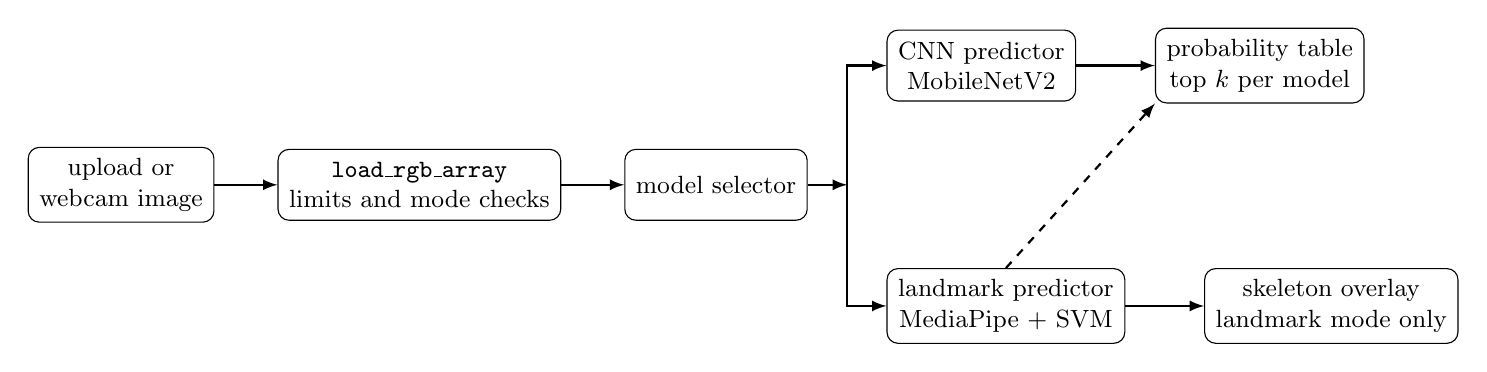
\begin{tikzpicture}[
  font=\small,
  box/.style={draw, rounded corners, align=center, inner sep=4pt, minimum height=9mm},
  arr/.style={-latex, thick},
  node distance=6mm and 8mm
]
\node[box] (input) {upload or\\webcam image};
\node[box, right=of input] (load) {\texttt{load\_rgb\_array}\\limits and mode checks};
\node[box, right=of load] (select) {model selector};
\node[box, above right=6mm and 10mm of select] (cnn) {CNN predictor\\MobileNetV2};
\node[box, below right=6mm and 10mm of select] (lm) {landmark predictor\\MediaPipe + SVM};
\node[box, right=10mm of cnn] (table) {probability table\\top $k$ per model};
\node[box, right=10mm of lm] (overlay) {skeleton overlay\\landmark mode only};
\draw[arr] (input) -- (load);
\draw[arr] (load) -- (select);
\draw[arr] (select.east) -- ++(5mm,0) coordinate (split);
\draw[arr] (split) |- (cnn.west);
\draw[arr] (split) |- (lm.west);
\draw[arr] (cnn) -- (table);
\draw[arr] (lm) -- (overlay);
\draw[arr, dashed] (lm.north) -- (table.south west);
\end{tikzpicture}%
}
\caption{The path of one request through the local app. The model selector decides which branches run; in \texttt{both} mode both run and the result table holds one block per model. The three honesty notes under the table are read from \texttt{configs/app.yaml}, and no image leaves the machine.}
\label{fig:app-flow}
\end{figure}

\subsection{What the Demo Shows and What It Does Not}

Table~\ref{tab:inference-demo} shows one image per letter through both predictors, using the top-1 result. The two models agree on A and B. On Z they differ: the CNN predicts Z, while the landmark model finds no hand in \texttt{Z1.jpg} and says so instead of guessing.

\begin{table}[h]
\centering
\caption{One image per letter through both predictors (top-1 result and probability).}
\label{tab:inference-demo}
\begin{tabular}{llll}
\hline
Image & CNN & Landmark model & Agree? \\
\hline
\texttt{A1.jpg} & A (0.811) & A (0.853) & yes \\
\texttt{B1.jpg} & B (0.953) & B (0.698) & yes \\
\texttt{Z1.jpg} & Z (0.963) & no hand detected & -- \\
\hline
\end{tabular}
\end{table}

The demo does not change the limits of the models. Both were trained on ASL fingerspelling, so no PSL accuracy is claimed. The scores are optimistic for the reasons in Section~\ref{sec:limitations}: 70.0\% of the test images have a same-class training image within 8 bits. The landmark model answers only when MediaPipe finds a hand, which happened for 69.9\% of the test images, and the array route used by the app can change a few results compared with the file route (Section~\ref{sec:landmark-inference}). Letters signed with movement, J and Z, cannot be captured from a single frame. The app is a demonstration of the trained models, not a claim of field accuracy.

\section{Landmark Inference in the Application}
\label{sec:landmark-inference}

This section describes how the trained SVM of Section~\ref{sec:landmark-models} is applied to one new image by the application, how closely that reproduces the saved results, and what limits it. The code is in \texttt{src/signbridge/inference/landmark\_predictor.py}. The class \texttt{LandmarkPredictor} follows the same interface as the CNN predictor: \texttt{predict(image, top\_k)} returns the \texttt{top\_k} most likely letters with their probabilities, sorted from highest to lowest.

\subsection{From Image to Letter}

\begin{enumerate}
\item \textbf{Input check.} The image must be a \texttt{uint8} RGB array of shape (height, width, 3). The shared helper rejects other types, shapes and oversized images with an \texttt{InvalidImage} error.
\item \textbf{Hand detection.} The MediaPipe hand landmarker (\texttt{models/hand\_landmarker.task}) runs in image mode for one hand with its default thresholds. These are the settings used to extract the training features, so inference sees hands the way training did. It returns 21 landmarks with $x$, $y$ and $z$.
\item \textbf{Normalisation.} The wrist (landmark 0) is subtracted from every point, and the result is divided by the distance from the wrist to the base of the middle finger (landmark 9). This gives the 63 features of Section~\ref{sec:landmark-models}, which no longer depend on where the hand is in the picture or how large it is. The function is a copy of \texttt{data\_scripts/features/landmarks.py}, because that folder is not part of the installed package; a unit test checks that both give identical output. The features are cast to 32-bit floats, as in the cached training features.
\item \textbf{Classification.} The saved pipeline standardises the features and applies the SVM ($C=100$, $\gamma=0.01$), whose probabilities come from \texttt{CalibratedClassifierCV}. The 26 probabilities are sorted and the first \texttt{top\_k} are returned.
\end{enumerate}

All paths come from \texttt{configs/app.yaml}. The two models are loaded once when the predictor is created and reused for every image; a lock allows only one MediaPipe call at a time. If MediaPipe finds no hand, or the landmarks are not finite or have zero hand size, the predictor raises \texttt{NoHandDetected}. We chose an exception over an empty list or a guess so that the application cannot mistake ``no answer'' for an answer. A second function, \texttt{draw\_landmarks}, draws the 21 points and their connections on a copy of the image, and returns nothing when no hand was found.

\textbf{Colour order.} The predictor expects RGB and never converts colours. OpenCV frames are BGR and must be converted by the caller; passing BGR would not raise an error but would change the pixels MediaPipe sees.

\subsection{Reproducing the Saved Results}

We ran the predictor on the 1{,}090 test images whose predictions are saved in \texttt{reports/predictions/\allowbreak landmark\_svm\_test.npz} and compared the 26 probabilities of each image.

\begin{table}[h]
\centering
\caption{The predictor compared with the saved test predictions (1{,}090 images).}
\label{tab:landmark-inference-check}
\begin{tabular}{lrrr}
\hline
Image route & No hand & Top-1 differs & Probability differs by $>0.001$ \\
\hline
File path (as in training) & 0 & 0 & 0 \\
NumPy array (as in the app) & 6 & 6 & 135 \\
\hline
\end{tabular}
\end{table}

When the predictor reads the file with MediaPipe's own reader, as the feature extraction did, it reproduces the saved predictions on every image. The application, however, passes a NumPy array that was decoded with Pillow. In a controlled check, the two decoders gave pixel values that differ by at most about 3 levels (mean about 0.07), and this was enough to change the result: on the array route MediaPipe missed the hand in 6 images, and among the 1{,}084 images where a hand was still found, 6 had a different top-1 letter and 135 had a probability that changed by more than 0.001. We did not change the interface to avoid this, because the application works with arrays. Results from the app can therefore differ slightly from the scores in this report.

\subsection{Limits of Landmark Inference}

\begin{itemize}
\item \textbf{No hand, no answer.} A hand was found in 69.9\% of the test images (Table~\ref{tab:landmark-detection}). For the other 470 images (30.1\%) the landmark model gives no prediction, whereas the CNN scores 0.983 accuracy on them (Section~\ref{sec:bias-check}). The first Z image of the dataset, \texttt{Z1.jpg}, is one of these cases.
\item \textbf{Fragile detection.} Detection depends on the image. Blur, occlusion, odd angles and tight crops can make MediaPipe miss the hand, and a tiny change in pixels can be enough, as the array route above shows.
\item \textbf{One hand, one frame.} The predictor runs in image mode on one hand per image. It cannot use motion, so the letters J and Z, which are signed with a movement, cannot be captured by a single frame (Section~\ref{sec:limitations}).
\item \textbf{Silent colour errors.} Because the predictor does not convert colours, a BGR frame from OpenCV gives wrong landmarks without an error message.
\item \textbf{Optimistic scores.} The scores of the model are optimistic for the reasons given in Section~\ref{sec:limitations}, and they describe American Sign Language only.
\item \textbf{Linux deployment.} MediaPipe needs the system libraries \texttt{libegl1} and \texttt{libgles2}; our continuous-integration run failed until they were installed.
\end{itemize}
\section{Deployment and Local Operation}
\label{sec:deployment}

The application is deployed locally. There is no hosted instance, no public link and no server deployment: a person who wants to use it runs it on their own machine. This is a deliberate limit, not a missing step. The models were trained on a public ASL dataset and the app is a demonstration, so putting a public endpoint on it would invite use on real signers before the PSL data, the signer-wise split and the field testing exist. The three screenshots in this section are safe figure slots: each one becomes a real screenshot when the image file is added to \texttt{reports/figures/}, and until then the report prints a red placeholder that names the missing file (owner: Anas).

\subsection{What a User Needs}

\begin{itemize}
\item Python 3.11.
\item The application requirements: \texttt{pip install -r requirements.txt} installs the shared pins, the CPU builds of PyTorch and torchvision, and Gradio. \texttt{pip install -e .} installs the package itself.
\item The model files, which are not in Git because they are binary: \texttt{models/cnn\_best.pt}, the three files in \texttt{models/landmark/} and \texttt{models/hand\_landmarker.task}. The README section ``Model weights'' gives the download links and the exact destinations.
\item A machine with a browser. No GPU is required; the CNN and the landmark models run on the CPU.
\end{itemize}

The whole application is one command from the repository root:

\begin{verbatim}
python app/app.py
\end{verbatim}

The server binds to \texttt{127.0.0.1} on port 7860, so it is reachable only from the same machine. The setting is in \texttt{configs/app.yaml} under \texttt{server}, together with \texttt{share: false}; the app never calls the public-link option. Changing the host to \texttt{0.0.0.0} would expose the app on the local network, and that is outside the scope of this project.

\subsection{Startup and Failure Behaviour}

The predictors are built on first use and cached, so the first prediction after a start is slower than the rest; the CNN loads its checkpoint once and the landmark predictor loads MediaPipe once. The app does not pre-load both models at start, so a user who only needs the CNN does not pay for MediaPipe.

Every failure becomes one readable line instead of a traceback:

\begin{itemize}
\item an upload above 20 MiB is refused by Gradio's upload limit (\texttt{max\_file\_size} from the settings) before the app sees it, and an image with a side above 4000 pixels is refused by \texttt{load\_rgb\_array}; neither is shrunk, because a resize would change what the model sees. The command-line tool reports the same two limits as \texttt{InvalidImage} errors;
\item a file that is not an image is refused by the uploader, and the server stays up; the command-line tool prints ``Could not read the image file'';
\item a missing checkpoint or a missing landmark file produces a \texttt{ModelNotFound} message that points to the README;
\item the landmark model on an image with no visible hand produces ``No hand detected: the landmark model needs a visible hand. Switch to the CNN, which does not need one.'';
\item a missing optional module produces a \texttt{PredictorUnavailable} message, and the rest of the interface still works.
\end{itemize}

The same checks live in the command-line tool, which reads the same \texttt{configs/app.yaml}, so the two entry points cannot drift apart.

\subsection{Screenshots}

The three slots below read their image from \texttt{reports/figures/} (owner: Anas). Until a file exists, the report prints a red placeholder that names the missing file, so the compiled PDF never hides a missing screenshot.

\safefigure{screenshot_upload.png}{The upload panel with a CNN prediction: the chosen image, the model selector, the number of predictions and the probability table. The model selector is set to \texttt{cnn}.}{fig:app-upload}

\safefigure{screenshot_both_models.png}{The \texttt{both} setting on \texttt{A/A1.jpg}: the CNN returns A (0.811) and the landmark SVM A (0.853), with the 21-point skeleton drawn over the image, so a reader can compare the two answers directly.}{fig:app-both-models}

\safefigure{screenshot_no_hand.png}{The landmark mode on an image with no visible hand: the result line says that the landmark model needs a visible hand and points to the CNN, and the three honesty notes stay visible.}{fig:app-no-hand}

\subsection{Privacy and Image Handling}

The app is local, and the models run on the same machine: no image is sent to a remote server for prediction. Gradio still writes an uploaded file to its temporary folder before the app reads it; on Windows this is under \texttt{\%TEMP\%\textbackslash gradio}, one folder per file named after the file's content hash. The app does not set \texttt{delete\_cache}, so those copies are not removed when the server stops. In a check on this machine, eleven folders from earlier sessions were still present. On a shared computer a user should clear that folder after a session. The app keeps no account, database or prediction log, but it also has no privacy notice and no retention period, which is one more reason not to host it.

\subsection{Why There Is No Hosted Version}

Hosting would add three problems that this project cannot answer yet. First, a public endpoint would need a privacy notice and a retention policy for the images people upload, and the project has neither. Second, the models are trained on ASL with near-duplicate leakage between the splits (Section~\ref{sec:limitations}), so a public demo would present optimistic scores as if they were field accuracy. Third, the PSL data does not exist yet, so a hosted app would still answer in ASL while carrying a PSL name. Running locally keeps the claim small and true: a demonstration of two trained models on one machine, with the limits printed on screen.

\section{User Test}
\label{sec:user-test}

A small test of the application was planned with three to five participants, about ten minutes each, following \texttt{docs/user\_test\_plan.md}. Each participant would upload a letter photo, show a letter to the webcam, upload an image with no hand, try a closed-fist letter in both model modes, and look for the note that says the models were trained on ASL. The observer would record what the app showed, whether the answer matched a printed ASL chart, and where the participant hesitated. The plan reports no percentages, because with three to five people a count of successes is not a rate.

The test was not carried out before this report was written. No participant took part, no session was recorded and no usability result is reported here. The plan, its consent line and its recording table are in the repository; running the test remains future work. The consent line still asks the team to state what the app does with uploaded images before the first session, and Section~\ref{sec:deployment} records what was measured: an upload is written to Gradio's temporary folder and is not deleted when the app stops.

\section{Limitations}
\label{sec:limitations}

\subsection{The Data Is American Sign Language}

The only large labelled dataset available to the project is the ASL Alphabet dataset. Every reported result in Deliverable~2 therefore describes American Sign Language, not Pakistan Sign Language. The two are different sign languages with different hand shapes, so the trained CNN cannot be used as a PSL recogniser and its scores do not transfer to PSL. The ASL baseline is used to build, train and compare the pipeline, not to make a claim about PSL accuracy.

\subsection{No PSL Photographs}

At the time of writing the team has collected 0 PSL photographs from 0 volunteers. The PSL letter set is also not final: published sources report 34 to 37 letters, and the current label map contains the 26 ASL letters A to Z. A PSL model, a PSL test set and any statement about PSL performance are therefore outside what this deliverable can show.

\subsection{A Subset of the Available Images}

Training does not use all 87{,}000 images of the ASL baseline. The shared split uses 400 cleaned images per class (10{,}400 in total, 7{,}280 in train, 280 per class in train) chosen by the data lead, and no per-class cap is applied at training time. This keeps tuning and final training feasible on the available hardware, but it reduces the variety the model sees and makes the results depend on which images were kept.

An existing PSL image dataset, UAlpha40 (CC BY 4.0, 36 static signs), is a candidate for PSL work in later deliverables; its folder structure and subject IDs have not been checked, and it was not used for any result in this report.

\subsection{Frames and Signers Are Not Independent}

The ASL baseline consists of video frames, and the number of distinct signers behind the dataset has not been verified. The shared split was generated by running the data lead's pipeline (\texttt{data\_scripts.build\_split\_pool} followed by \texttt{signbridge.data.splits}) on the ASL training folder with the committed configuration (seed 42, 400 images per class), giving 10{,}400 images in total (7{,}280 train, 1{,}560 validation and 1{,}560 test). Near-duplicates were removed from the split pool at a Hamming distance of 3 bits, the remaining images were placed in leader groups at 10 bits, and every group was assigned whole to one split, so the per-class shares are exactly 70/15/15. Grouping reduces leakage but does not remove it. Using the same 64-bit difference hash as the cleaning scripts, 21.0\% of validation and 20.3\% of test images have a training image of the same class within 4 bits; the figures rise to 49.9\% and 47.2\% within 6 bits, 73.4\% and 70.0\% within 8 bits, and 87.4\% and 87.4\% within 10 bits. The closest training neighbour is 4 bits away in both splits. The cause is that leader grouping bounds each image's distance to its own group leader, not the distance between every pair of images in different groups. The reported validation and test scores are therefore optimistic, and they are not an estimate of accuracy on new signers. One class also has a single group holding 43 of its 400 images (10.75\%), slightly above the 10\% target used when choosing the setting; all other classes are below 10\%.

\subsection{Small Compute Budget}

The long runs were done on a free cloud T4 GPU, not on the project laptop. The tuning search ran 12 trials of 3 epochs, about 26 minutes of training in total, and the final run stopped after 9 of the 12 configured epochs, about 6 minutes. The GPU took about 0.15 seconds per batch at $224\times224$ and batch size 32, against the 3.2 seconds per batch measured on the CPU, which is why the search and the final run were moved off the laptop. A larger budget would allow more trials, repeated seeds to measure run-to-run noise, more epochs or a larger subset. The split still uses 280 training images per class, so the results are limited by the data as well as by the search.

\subsection{Static Letters Only}

The system classifies a single image of one hand. It does not use motion, temporal information, two-handed signs, words or sentences, and it does not translate between PSL and text or speech. Letters that require movement are outside its scope.

\subsection{The CNN Always Gives an Answer}

The CNN is a 26-way classifier: it returns a probability for each letter and has no class for ``no hand''. It therefore answers every picture it is given. In an informal check before the user test --- twelve pictures taken by two people in one room, one picture per case, not a measurement and not part of any score in this report --- four pictures with no hand at all (a face, a wall and bed frame, party decorations, and a face partly covered by a hand) each received a letter from the CNN, once with a probability of 0.867, while the landmark model returned no hand in all four. This is not the same as the 0.983 accuracy reported for images in which MediaPipe found no hand (Section~\ref{sec:bias-check}): in those images a hand is present and the landmarker missed it, so they say nothing about a picture with no hand in it.

The landmark model's refusal is not a reliable hand detector either. In the same check it returned no hand for the picture in which a hand covered a face, although a hand was there. That is the detection limit already measured on the test set, where a hand was found in 69.9\% of the images (Table~\ref{tab:landmark-detection}).

A high probability is not a sign that the answer is right. In the same check, of the six pictures that showed a chart letter, each model's top answer was correct in one picture; the letter A, shown twice by two different hands, was outside both models' top three both times; one picture had the correct letter in second place, 0.0002 behind the first; and the landmark model gave 0.904 to a wrong letter. The letter L, shown by two hands, was read correctly by a different model each time. We do not turn these observations into rates, and the app does not add a confidence threshold: choosing one would need calibrated probabilities from more than twelve pictures, and a threshold would hide a wrong answer rather than remove it. A rejection option for the CNN would need a separate hand detector or a calibrated score and is left to later work. The no-hand message in the app therefore belongs to the landmark model, which is the only one that can refuse.

\subsection{No Demographic Bias Assessment}

The dataset has no demographic labels, and no PSL volunteers were photographed. It is therefore not possible to measure whether the recogniser performs differently across age, gender, skin tone or signing background. The bias discussion in this report is limited to what can be measured without those labels, such as performance by letter and by image brightness or blur, and it cannot support a claim of fairness.

\section{Contributions}
\label{sec:contributions}

The contribution table is produced mechanically from the Git history, not written by hand. \texttt{tools/contribution\_table.py} reads \texttt{configs/modules.yaml}, which maps each project module to one owner and to a set of path globs. For every module it runs

\begin{quote}
\texttt{git log -{}-use-mailmap -{}-no-merges -{}-format=\%aN <revision> -{}- <paths>}
\end{quote}

on the \texttt{main} branch and counts the commits per author. Merge commits are excluded, and commits that exist only on unmerged branches are not reachable from \texttt{main} and are therefore not counted. The option \texttt{-{}-use-mailmap} makes Git group the author aliases listed in \texttt{.mailmap} under one canonical name, so the same person does not appear twice because of a different spelling of their name or a different e-mail address. The script writes both \texttt{reports/contribution\_table.csv} and the LaTeX table \texttt{reports/contribution\_table.tex}; the latter is included below.

\IfFileExists{../../reports/contribution_table.tex}{%
  \begin{table}[htbp]
  \centering
  \caption{Non-merge commits reachable from \texttt{main}, grouped by module and author through \texttt{.mailmap}.}
  \label{tab:contributions}
  \resizebox{\linewidth}{!}{\begin{tabular}{lll}
\hline
Module & Owner & Authors (commits) \\
\hline
shared\_config & Anas & Anas Rashid (6), Aliza (5), Fatima Asif (1) \\
project & Anas & Anas Rashid (14), Fatima Asif (1) \\
readme & Shared & Anas Rashid (14), Aliza (3) \\
protocol & Aliza & Aliza (7), Anas Rashid (3) \\
download & Anas & Anas Rashid (1) \\
cleaning & Aliza & Aliza (5), Anas Rashid (2) \\
raw\_eda & Aliza & Aliza (5), Anas Rashid (2) \\
landmarks & Fatima & Fatima Asif (16) \\
labels\_and\_images & Fatima & Fatima Asif (3) \\
manifest & Aliza & Aliza (2) \\
splits & Aliza & Aliza (6), Anas Rashid (2) \\
evaluation & Aliza & Aliza (15), Anas Rashid (2), Fatima Asif (1) \\
landmark\_models & Fatima & Fatima Asif (26), Anas Rashid (3) \\
cnn\_model & Anas & Anas Rashid (5) \\
cnn\_training & Anas & Anas Rashid (6) \\
cnn\_tuning & Anas & Anas Rashid (1) \\
inference & Anas & Anas Rashid (11) \\
tools & Anas & Anas Rashid (13) \\
overview & Aliza & Aliza (2) \\
user\_test & Aliza & Aliza (1) \\
report & Anas & Anas Rashid (45), Aliza (8), Fatima Asif (7) \\
tests & Shared & Anas Rashid (21), Fatima Asif (17), Aliza (16) \\
\hline
\end{tabular}
}
  \end{table}
}{%
  \todobox{The contribution table is missing. It will be generated by \texttt{tools/contribution\_table.py} after the model commits are merged into \texttt{main} and the author aliases in \texttt{.mailmap} are confirmed.}
}

\section{Conclusion and Future Work}
\label{sec:conclusion}

\subsection{What We Did}

We built and evaluated two recognisers for the 26 letters A to Z: a MobileNetV2 CNN and landmark models that classify 21 MediaPipe hand points. The data was split by groups of look-alike images (10{,}400 images, 280 train, 60 validation and 60 test per letter). On the 1{,}560 test images the CNN scored 0.9795 accuracy and 0.9795 macro-F1. The landmark models answered the 1{,}090 test images (69.9\%) in which a hand was detected. On those images the CNN scored 0.9780 accuracy and the SVM, the landmark model chosen by the validation rule, 0.9688. The SVM and the MLP differ by less than one validation image, so we cannot tell them apart.

\subsection{What the Results Do Not Show}

\begin{itemize}
  \item \textbf{They are about ASL, not PSL.} We trained on the ASL alphabet because we had no PSL photographs. No score here says anything about PSL.
  \item \textbf{They are optimistic.} 70.0\% of test images have a training image of the same letter within 8 bits of the image hash. The data has no signer labels, so we cannot say whether the same people appear in training and test. The scores are not an estimate of accuracy on new signers.
  \item \textbf{They are not a claim of robustness or fairness.} We found no clear difference by blur or hand detection and a small pattern by brightness. The dataset has no demographic labels, so we say nothing about skin tone, gender or signer.
  \item \textbf{The comparison is narrow.} The CNN is ahead of the SVM by 10 images out of 1{,}090. We ran no significance test, and the landmark models cannot answer the 30.1\% of test images with no detected hand.
\end{itemize}

\subsection{Future Work}

These are the steps we think would make the work meaningful. We have not started any of them.
\begin{enumerate}
  \item \textbf{Collect PSL photographs with signer labels.} Photograph PSL signers with their consent and record a signer identifier for every image, after a PSL user has confirmed the letter set (34 to 37 letters are reported in the sources we cite).
  \item \textbf{Split by person.} With signer labels, split by signer so that no person appears in more than one split. This is the only way to estimate accuracy on new people.
  \item \textbf{Check an existing PSL dataset.} UAlpha40 is a candidate. Its folder structure, subject identifiers and suitability have not been checked, and we used it for no result.
  \item \textbf{Measure uncertainty properly.} Our bootstrap intervals resample images, not groups, so they are too narrow. Resampling signers or groups would give honest intervals.
  \item \textbf{Assess fairness only with consent.} If participants agree to share attributes such as age or skin tone, check whether accuracy differs between groups. We cannot do this without such labels.
  \item \textbf{Go beyond single letters.} Letters that need motion, words and sentences need video and much more data, and are outside the scope of this project.
\end{enumerate}


\bibliographystyle{plain}
\begingroup
\raggedright
\bibliography{references}
\endgroup

\end{document}
